\documentclass{article}
\usepackage[T2A]{fontenc}
\usepackage[utf8]{inputenc}
\usepackage[russian]{babel}
\usepackage{amsmath,amssymb,amsthm,enumitem, empheq}
\usepackage{exercise}
\usepackage{pgf,tikz,tkz-tab}
\usepackage{pgfplots}
\usepackage{graphicx}
\usepackage{circuitikz}
\usepackage{hyphenat}
\usepackage{multirow}
%\usepackage{pdfpages}

\usetikzlibrary{arrows}
\usetikzlibrary{circuits}

\title{Теория вероятностей}
\author{Ле Куок Зунг}
\date{\today}

\theoremstyle{definition}
\newtheorem*{exercise}{Упражение}
%\DeclareMathOperator{\tg}{tg}

\begin{document}
	\maketitle
	\section*{Занятия 2}
\begin{exercise}[1] Десять команд случайным образом (по жребию) разбиваются на две разные подгруппы. 
	
	$| \Omega | = C^5_{10} C^5_5$
	
	\begin{enumerate}
		\item [(a)] Выбрать место для 2 сильнейших команд: 2 \\ Выбрать 4 команда для подгруппы 1: $C^4_8$ \\ Выбрать 4 команда для подгруппы 2: $C^4_4$ \\ Ответ: $\frac{2 C^4_8 C^4_4}{C^5_{10} C^5_5} = \frac{5}{9}$
		\item [(б)] Выбрать подгруппу для 2 команда: $C^1_2$ \\ Выбрать больше 3 команда этой группы: $C^3_8$ \\ Ответ: $\frac{C^1_2 C^3_8}{C^5_{10} C^5_5} = \frac{4}{9}$
		\item [(в)] Выбрать больше 3 команда первой группы: $C^3_8$ \\ Выбрать 5 команд второй группы: $C^5_5$ \\ Ответ: $\frac{C^3_8 C^5_5}{C^5_{10} C^5_5} = \frac{2}{9}$
	\end{enumerate}
\end{exercise}

\begin{exercise}[2]
	\begin{enumerate}
		\item [(а)] $| \Omega | = C^3_{52}$ \\ Выбрать тройку $C^1_4$, семарку $C^1_4$, туз $C^1_4$ \\ Ответ: $\frac{C^1_4 C^1_4 C^1_4}{C^3_{52}} = \frac{16}{5525}$
		\item [(б)] $| \Omega | = A^3_{52}$ (так как мы выберем последовательные карты) \\ Для три любых карт существует только один заказ, поэтому нужно выбрать атрибут первой карты $C^1_4$, второй $C^1_4$, третьей $C^1_4$ \\ Ответ: $\frac{C^1_4 C^1_4 C^1_4}{A^3_{52}} = \frac{8}{16575}$
	\end{enumerate}
\end{exercise}

\begin{exercise}[3]
	\begin{tikzpicture}
		\draw (-4,0) -- (4,0);
		\filldraw [black] (-4,0) circle (2pt) node[anchor=south]{$O$};
		\filldraw [black] (-2,0) circle (2pt) node[anchor=south]{$B$};
		\filldraw [black] (1.5,0) circle (2pt) node[anchor=south]{$C$};
		\filldraw [black] (4,0) circle (2pt) node[anchor=south]{$A$};
	\end{tikzpicture}
	
	Пусть $L$ - длина отрезка $OA$ \\ $x$ - длина отрезка $OB$ \\ $y$ - длина отрезка $BC$ \\ У нас есть: $\begin{cases}
		y < x \\ x +y < L \\ x > 0 \\ y > 0
	\end{cases}$
	
	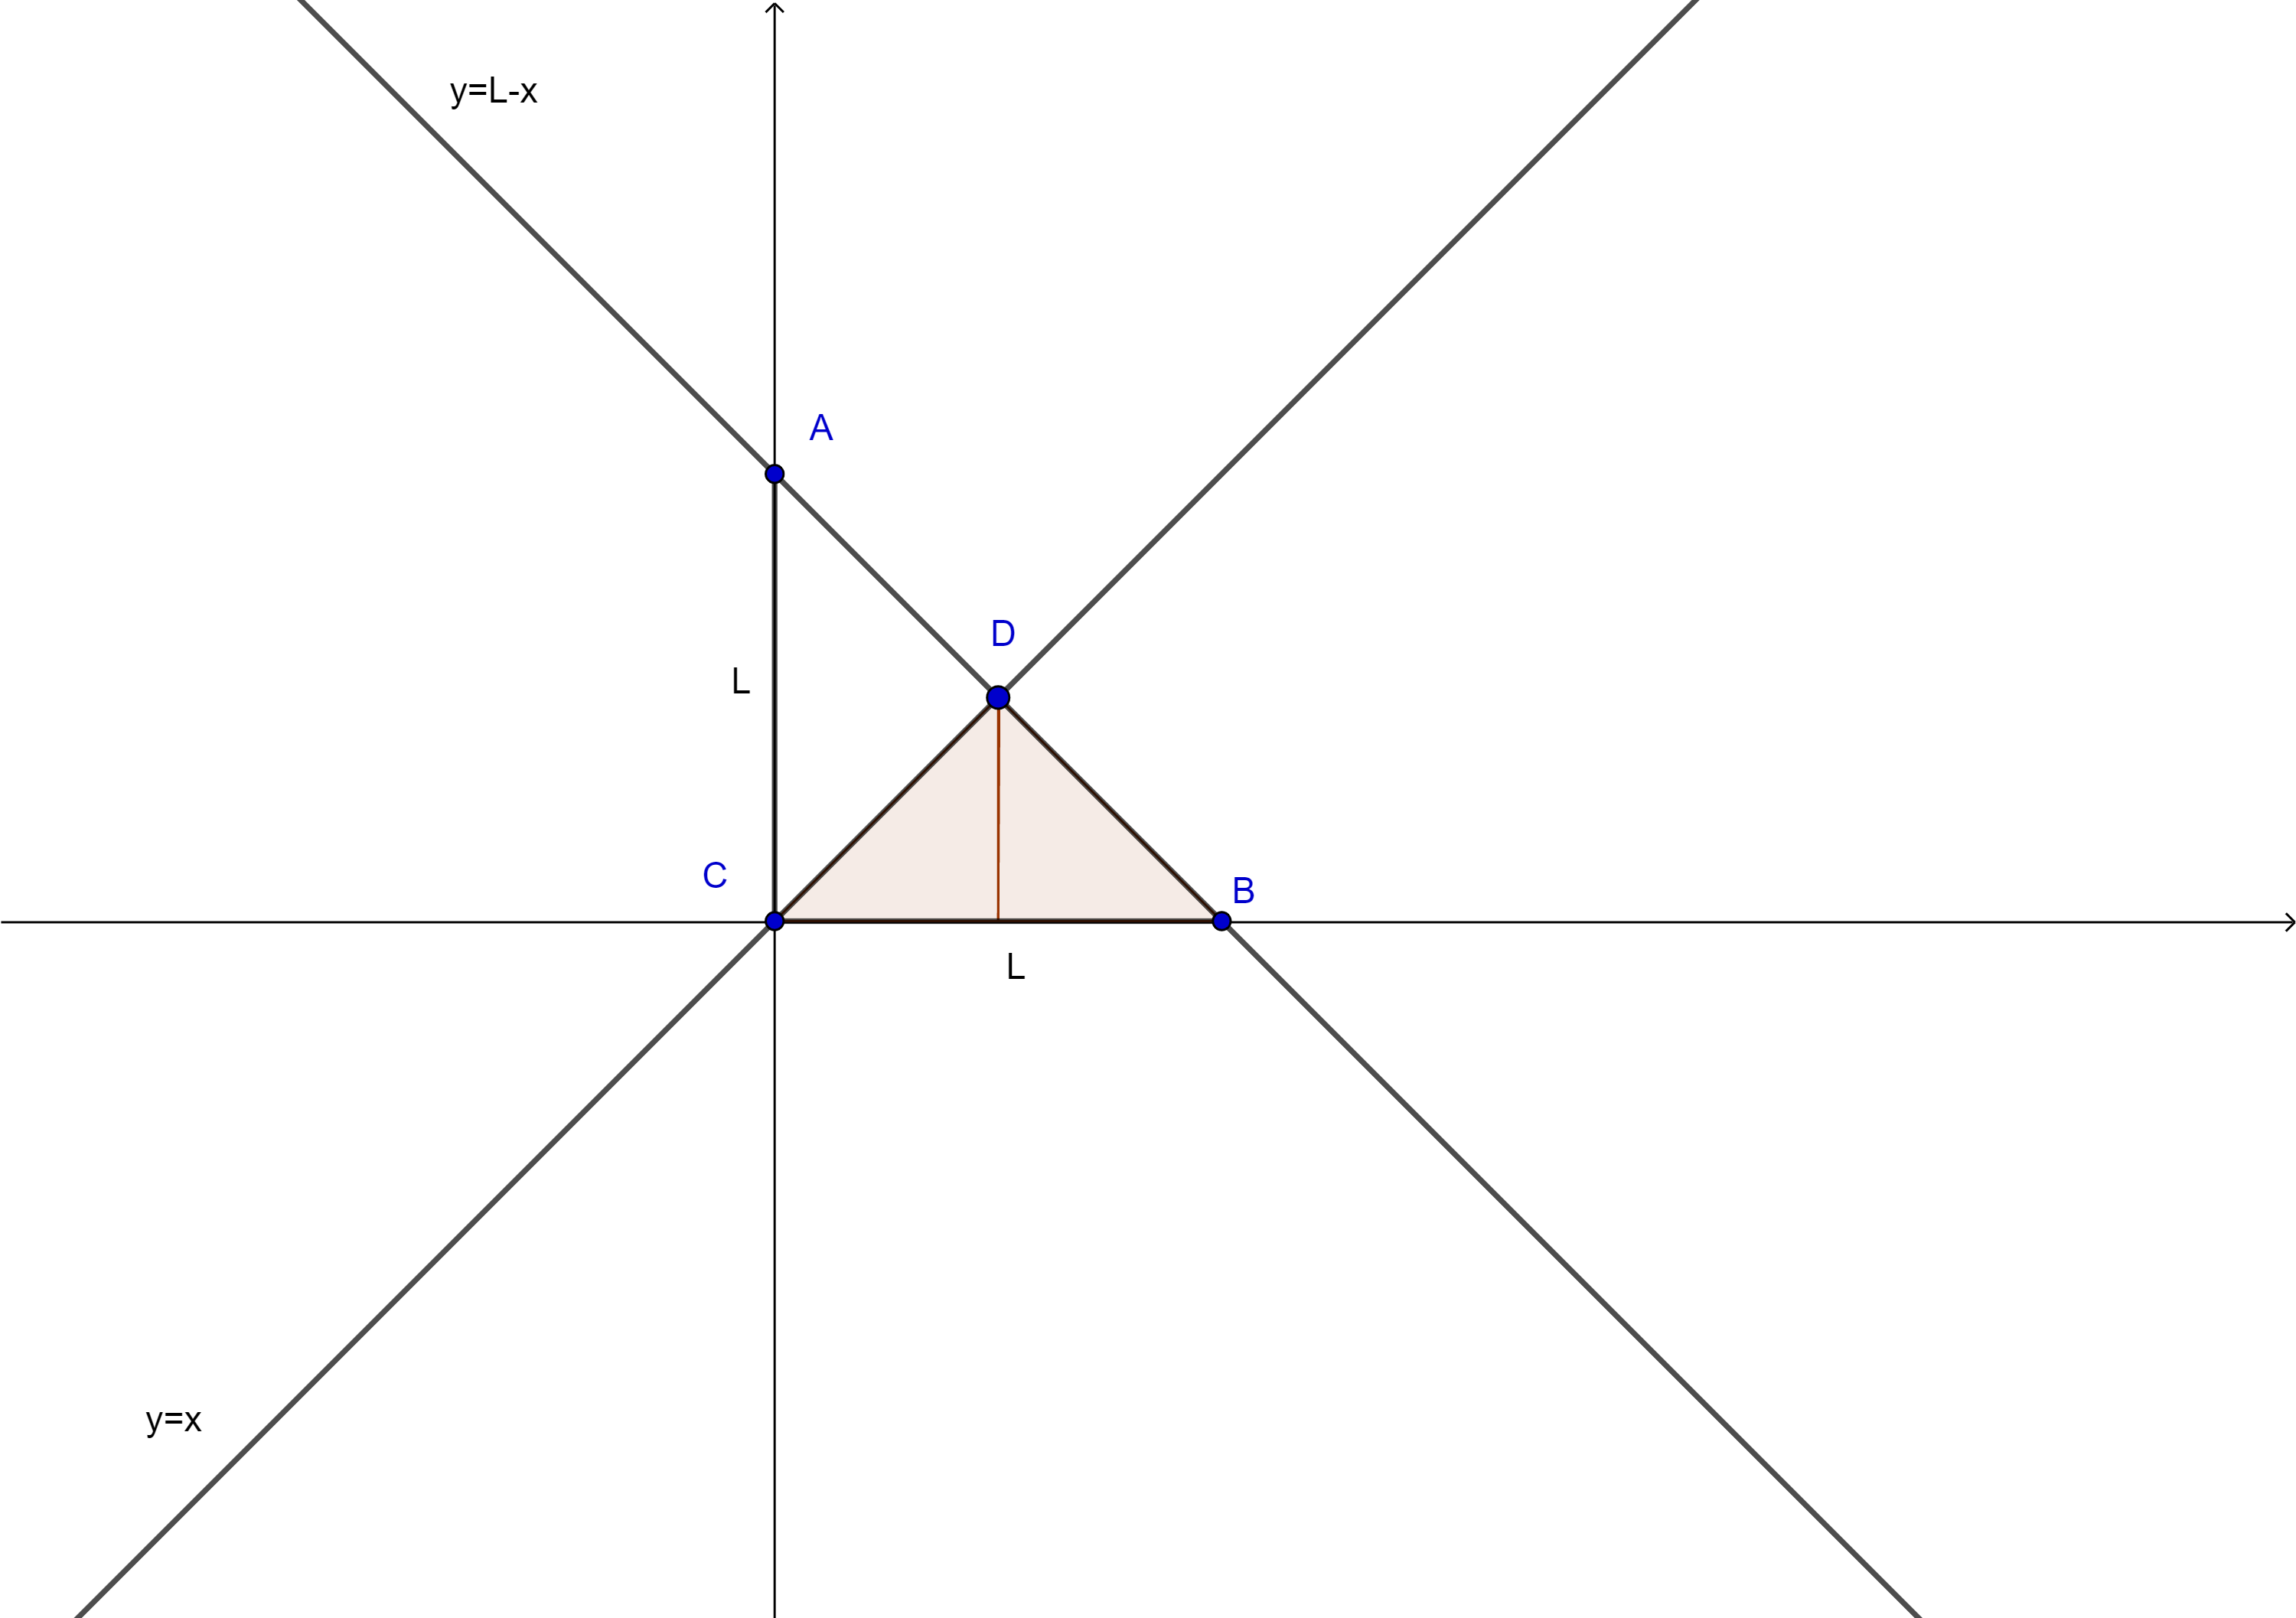
\includegraphics[width=\textwidth]{exercise3-2.png}	
	
	Здесь, $| \Omega | = \frac{L^2}{2}$, а вероятность, которая удовлетворяет условии: $\frac{L \cdot \frac{L}{2}}{2} = \frac{L^2}{4}$ \\ Ответ: $\frac{L^2}{4} : \frac{L^2}{2} = \frac{1}{2}$
\end{exercise}

\begin{exercise}[4]
	$| \Omega | = 10!$ \\ Ответ: $\frac{1}{10!}$
\end{exercise}

\begin{exercise}[5]
	$| \Omega | = 8^4$
	\begin{enumerate}
		\item [(a)] Выбрать 4 этажа из 8: $A^4_8$ \\ Ответ: $\frac{A^4_8}{8^4} = \frac{105}{256}$
		\item [(б)] Этаж 6, 7, 8, 9, поэтому 4 этажа: $4^4$ \\ Ответ: $\frac{4^4}{8^4} = \frac{1}{16}$
		\item [(в)] 7 этажов: $7^4$ \\ Ответ: $\frac{7^4}{8^4} = \frac{2401}{4096}$
	\end{enumerate}
\end{exercise}

\begin{exercise}[6]
	$| \Omega | = 10^4=10000$
	\begin{enumerate}
		\item [(a)] Первое число имеет 9 вариантов (кроме 0). Другие числа имеют 10 вариантов \\ Ответ: $\frac{9 \cdot 10^3}{10^4} = 0,9$
		\item [(б)] Чтобы делится на 5, последнее число равно 0 или 5 \\ Ответ: $\frac{9 \cdot 10^2 \cdot 2}{10^4} = 0,18$
	\end{enumerate}
\end{exercise}

\begin{exercise}[7]
	$| \Omega | = C^{10}_{20}$ \\ Если билеты 1 и 2 не будет, тогда имеется 18 билетов, значит $C^{10}_{18}$ \\ Ответ: $\frac{C^{10}_{18}}{C^{10}_{20}} = \frac{9}{38}$
\end{exercise}

\begin{exercise}[8]
	$| \Omega | = C^4_{6+4+2} = C^4_{12}$ \\ Ответ: $\frac{C^4_{4+2}}{C^4_{12}} = \frac{1}{33}$
\end{exercise}

\begin{exercise}[9]
	$| \Omega | = 10!$ \\ 
	Рассмотрим 3 красного книги как 1, тогда у нас нес 8 книг. Найти места для 8 книг: $8!$ \\ 3 краного книга имеет $3!$ \\ Ответ: $\frac{8! 3!}{10!} = \frac{1}{15}$
\end{exercise}

\begin{exercise}[10]
	Каждая кость имеет 6 вариантов, поэтому $| \Omega | = 6^3$ \\ События А: кости выпадут разными гранями, то есть $6 \cdot 5 \cdot 4$ \\ Тогда, $P(A) = \frac{6 \cdot 5 \cdot 4}{6^3} = \frac{5}{9}$ \\ События B: на всех костях выпадет одинаковое число очков, то есть 6 чисел \\ Тогда $P(B) = \frac{6}{6^3} = \frac{1}{36}$
\end{exercise}

\begin{exercise}[11]
	У нас есть 5 пар ботинок, значит 10 ботинок. Поэтому $| \Omega | = C^2_{10}$ \\ Существуют 5 пар, то $P(A) = \frac{5}{C^2_{10}} = \frac{1}{9}$
\end{exercise}

\begin{exercise}[12]
	Тат как каждый участник может получит любый приз, поэтому $| \Omega | = 10^6$ \\ Данные 6 учасников получат по одному призу каждый, то $6!$ \\ Ответ: $\frac{6!}{10^6} = 0,00072$
\end{exercise}

\begin{exercise}[13]
	$| \Omega | = C^4_8 C^4_4$ \\ Выбрать 2 юношей и 2 девушек для группы 1: $C^2_4 C^2_4$ \\ Ответ: $\frac{C^2_4 C^2_4}{C^4_8 C^4_4} = \frac{18}{35}$
\end{exercise}

\begin{exercise}[14]
	\item [(a)] $P(A) = \frac{S_{\square}}{S_{\circ}} = \Big(\frac{2R}{\sqrt{2}}\Big)^2:(\pi R^2) = \frac{2}{\pi}$
	\item [(б)] $P(B) = \frac{S_{\triangle}}{S_{\circ}} = \Big[(R \sqrt{3})^2 \cdot \frac{\sqrt{3}}{4}\Big] : (\pi R^2) = \frac{3 \sqrt{3}}{4 \pi}$
\end{exercise}

\begin{exercise}[15] В течение суток к причалу независимо друг от друга
	
	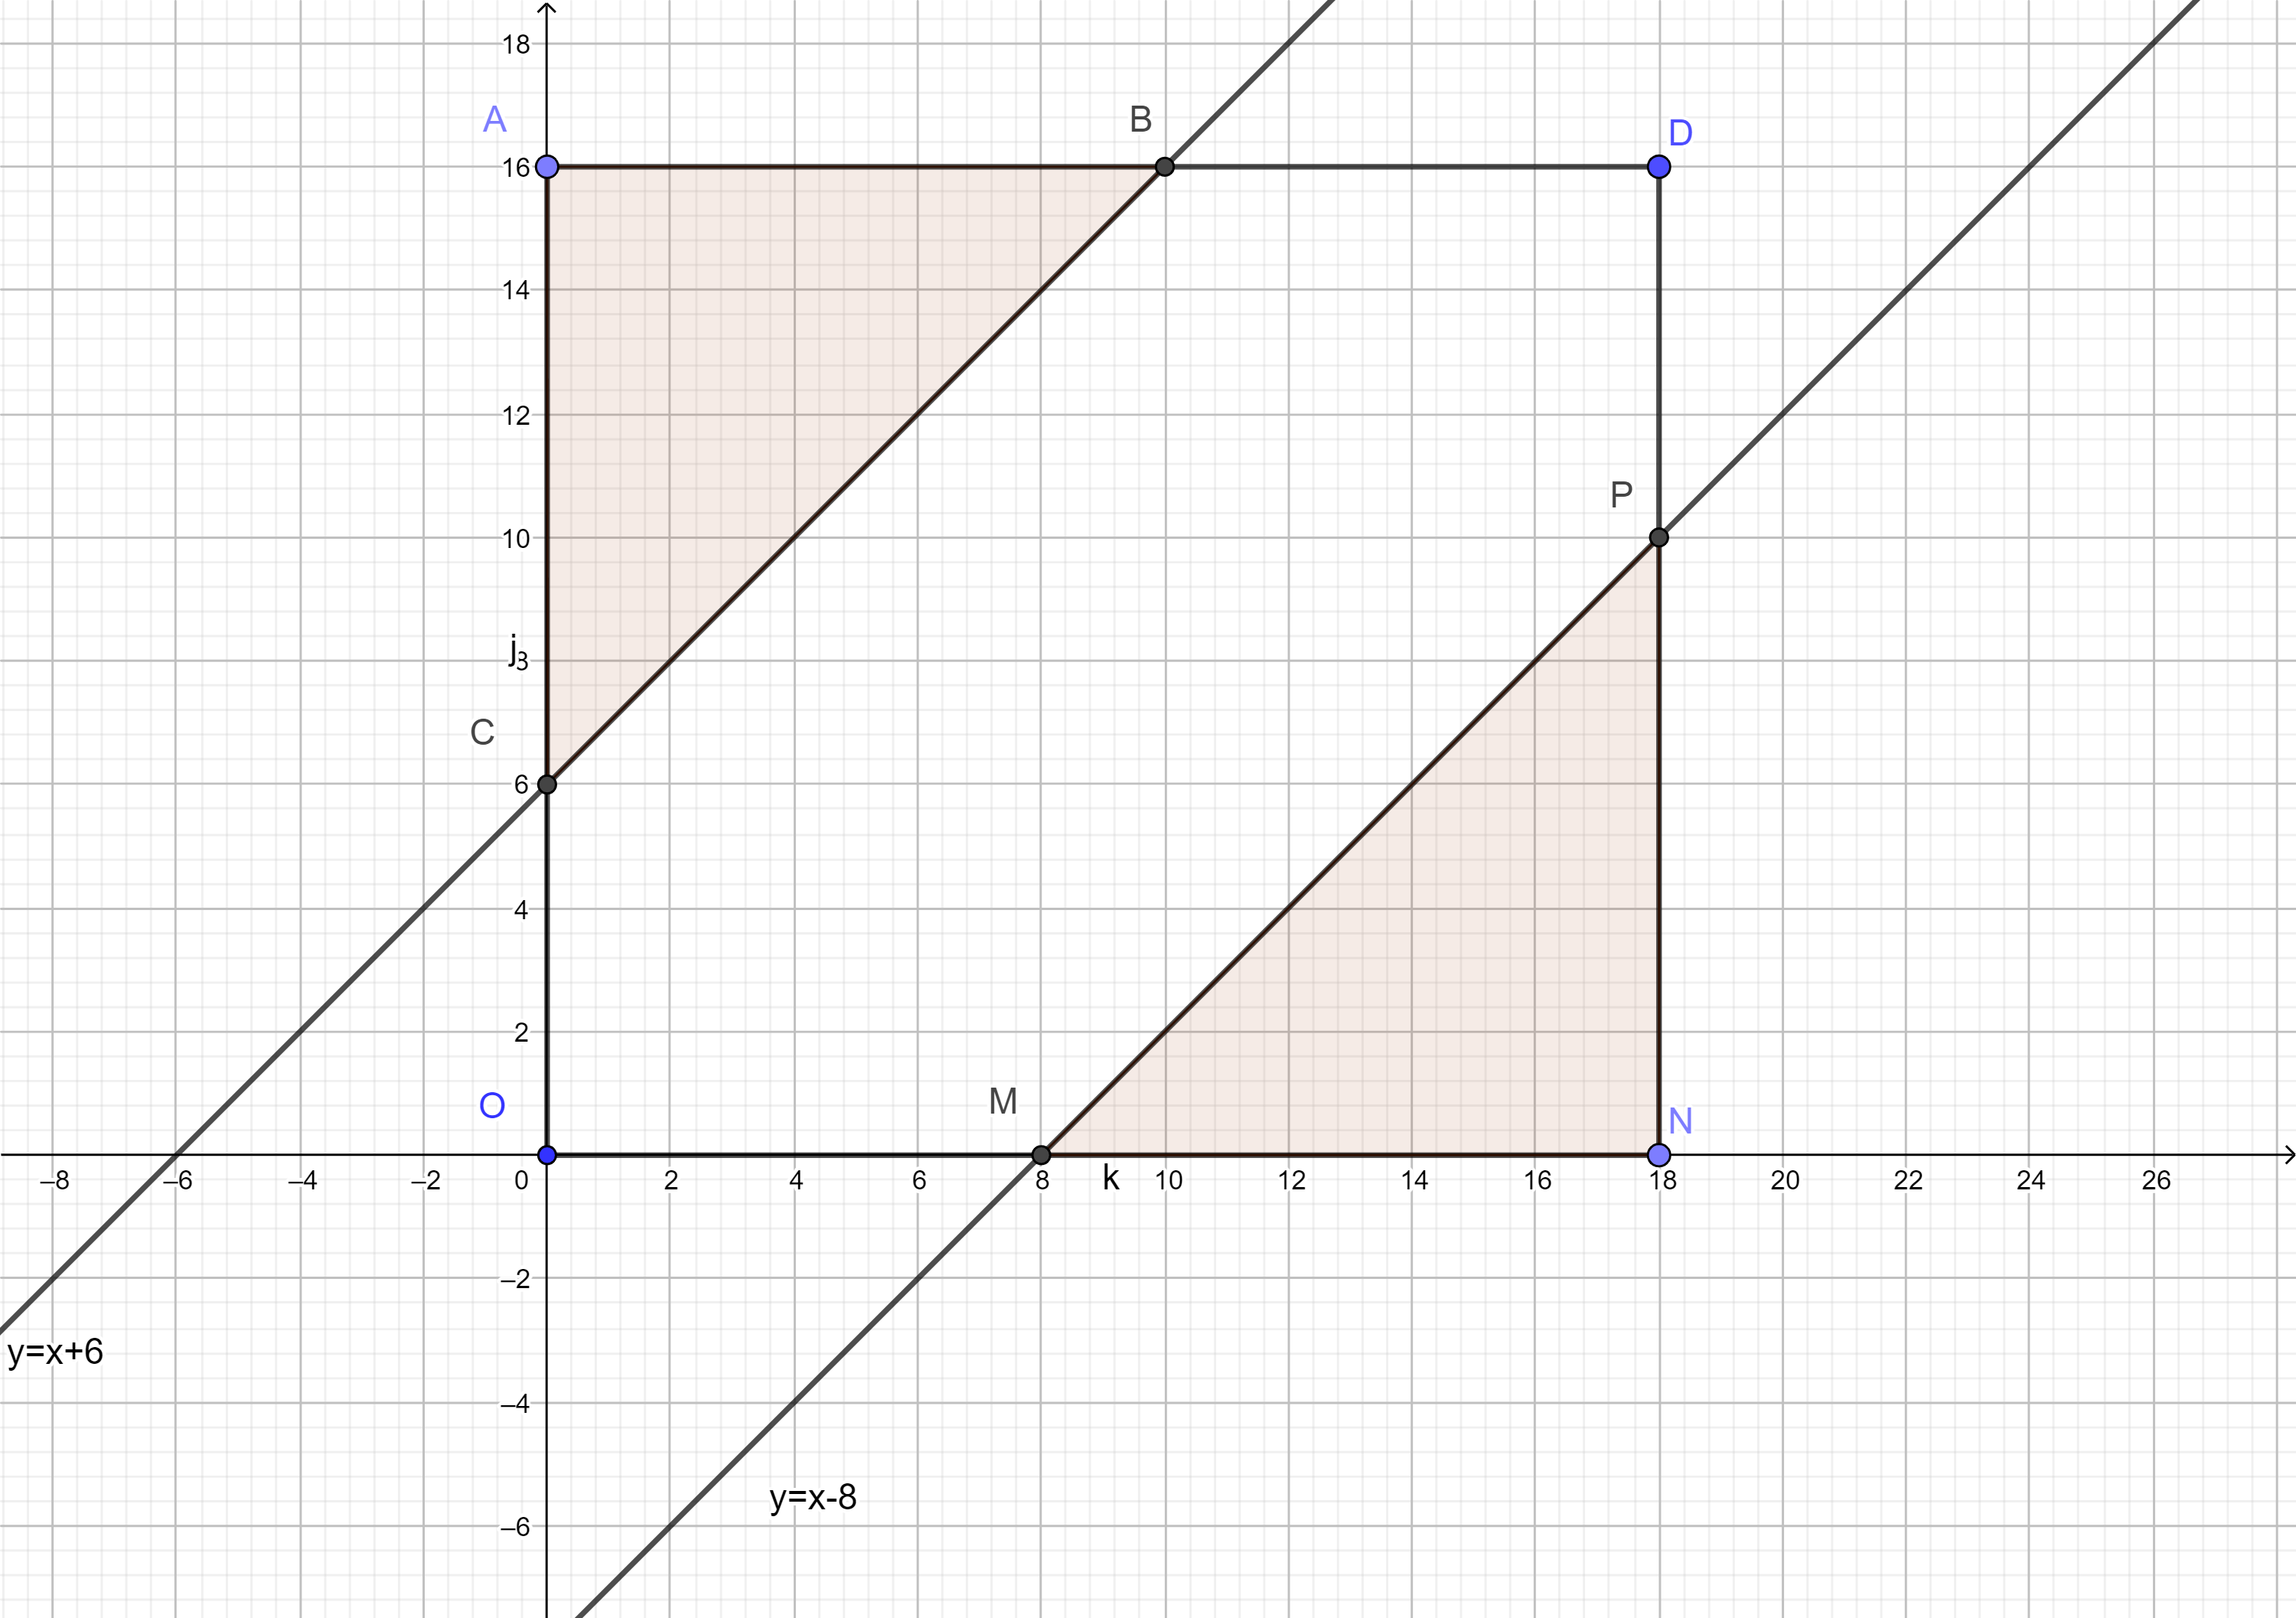
\includegraphics[width=\textwidth]{exercise15-2.png}
	
	Пусть $x$ - время первый сухогруз начинает разгрузиться и $y$ - время второй сухогруз начинает разгрузиться \\ Тогда, $x+6 \leq 24$ и $y+8 \leq 24 \Leftrightarrow x \leq 18$ и $y \leq 16$ \\ Cлучай 1: первый сухогруз начинает раньше чем второй, тогда $x+6 \leq y$ \\ Случай 2: второй сухогруз начинает раньше чем первый, тогда $y+8 \leq x$ \\ Получим $P(A) = \frac{S_{\triangle ABC} + S_{\triangle MNP}}{S_{ADNO}} = \Big(\frac{10 \cdot 10}{2} + \frac{10 \cdot 10}{2} \Big) : (16 \cdot 18) = \frac{25}{72}$ 
\end{exercise}
	\newpage
	\section*{Занятие 3}
\begin{exercise}[1]
	
	\begin{enumerate}
		\item [(a)] Пусть $A$ - вероятность безотказной работы
		
		\begin{circuitikz}
			\draw
			(0,1) to[] (1,1)
			(1,1) to[] (1,0)
			(1,1) to[] (1,2)
			(1,2) to[generic,l=$1$] (3,2)
			(1,0) to[generic,l=$2$] (3,0)
			(3,1) to[] (3,2)
			(3,1) to[] (3,0)
			(3,2) to[generic,l=$3$] (5,2)
			(3,0) to[generic,l=$4$] (5,0)
			(5,1) to[] (5,0)
			(5,1) to[] (5,2)
			(5,2) to[generic,l=$5$] (7,2)
			(5,0) to[generic,l=$6$] (7,0)
			(7,1) to[] (7,0)
			(7,1) to[] (7,2)
			(7,2) to[generic,l=$7$] (9,2)
			(7,0) to[generic,l=$8$] (9,0)
			(9,1) to[] (9,0)
			(9,1) to[] (9,2)
			(9,1) to[] (10,1)
			;
		\end{circuitikz}
		
		\begin{align*}
			\Rightarrow P(A) & = P(A_1 + A_2) P(A_3 + A_4) P(A_5 + A_6) + P(A_7 + A_8) \\ & = [1-(1-P(A_1))(1-P(A_2))] \cdot [1-(1-P(A_3))(1-P(A_4))] \\ & \times [1-(1-P(A_5))(1-P(A_6))] \cdot [1-(1-P(A_7))(1-P(A_8))] \\ & = (1-(1-0,8)(1-0,8))^4 \\ & \approx 0,85
		\end{align*}
	
		\item [(б)] Пусть $A$ - вероятность безотказной работы
		
		\begin{circuitikz}
			\draw
			(0,1) to[] (1,1)
			(1,1) to[] (1,0)
			(1,1) to[] (1,2)
			(1,2) to[generic,l=$1$] (3,2)
			(1,0) to[generic,l=$2$] (3,0)
			(3,1) to[] (3,2)
			(3,1) to[] (3,0)
			(3,1) to[generic,l=$3$] (5,1)
			(5,1) to[] (5,0)
			(5,1) to[] (5,2)
			(5,2) to[generic,l=$4$] (7,2)
			(5,0) to[generic,l=$5$] (7,0)
			(7,1) to[] (7,0)
			(7,1) to[] (7,2)
			(7,1) to[] (8,1)
			;
		\end{circuitikz}
		
		\begin{align*}
			P(A) & = P(A_1 + A_2) P(A_3) P(A_4 + A_5) \\ & = [1 - (1-P(A_1))(1-P(A_2))] \cdot P(A_3) \cdot [1-(1-P(A_4))(1-P(A_5))] \\ & = (1-(1-0,8)^2) \cdot 0,8 \cdot (1-(1-0,8)^2) \\ & = 0,73728 \approx 0,74
		\end{align*}
	
		\item [(в)] Пусть $A$ - вероятность безотказной работы
		
		\begin{circuitikz}
			\draw
			(0,2) to[generic,l=$1$] (5,2)
			(5,2) to[generic,l=$2$] (10,2)
			(1,2) to[] (1,0)
			(1,0) to[] (3,0)
			(3,0) to[] (3,1)
			(3,0) to[] (3,-1)
			(3,1) to[generic,l=$3$] (7,1)
			(3,-1) to[generic,l=$4$] (7,-1)
			(7,0) to[] (7,1)
			(7,0) to[] (7,-1)
			(7,0) to[] (9,0)
			(9,0) to[] (9,2)
			;
		\end{circuitikz}
	
		\begin{align*}
			P(A) & = P(A_1 A_2 + A_3 + A_4) \\ & = 1 - (1 - P(A_1 A_2) (1 - P(A_3)) (1 - P(A_4))) \\ & = 1 - (1 - P(A_1) P(A_2) (1 - P(A_3)) (1 - P(A_4))) \\ & = 1 - (1 - (0,8)^2 \cdot (1 - 0,8) \cdot (1 - 0,8)) \\ & = 0,9856 \approx 0,98
		\end{align*}
		
	\end{enumerate}
\end{exercise}

\begin{exercise}[2]
	Пусть $A$ - событие после 4 шара появится черный шар \\ $A_1, A_2, A_3$ - события выбрать белый шар в \textit{i-ый} раз \\ $A_4$ - событие выбрать черный шар в последний раз \\ $P(A) = P(A_1) P(A_2) P(A_3) P(A_4)$
	
	\begin{enumerate}	
		\item [(a)] $P(A_1) = P(A_2) = P(A_3) = \frac{7}{10}$ \\ $P(A_4) = \frac{3}{10}$ \\ $\Rightarrow P(A) = \Big(\frac{7}{10}\Big)^3 \cdot \frac{3}{10} = \frac{1029}{10000} = 0,1029$
		\item [(б)] $P(A_1) = \frac{7}{10}$, $P(A_2) = \frac{6}{9}$, $P(A_3) = \frac{5}{8}$ \\ $P(A_4) = \frac{3}{7}$ \\ $\Rightarrow P(A) = \frac{7}{10} \cdot \frac{6}{9} \cdot \frac{5}{8} \cdot \frac{3}{7} = \frac{1}{8}$
	\end{enumerate}
\end{exercise}

\begin{exercise}[3]
	Пусть $A$ - событие среди них окажется по меньше мере одна кость с шестью очками \\ Тогда, $\bar{A}$ - событие нет кости с шестью очками. То $\bar{A}$ имеет 28-7=21 вариантов \\ $| \Omega | = C^7_{28}$ \\ $\Rightarrow P(A) = 1-P(\bar{A}) = 1 - \frac{C^7_{21}}{C^7_{28}} = \frac{2966}{3289} \approx 0,9$
\end{exercise}

\begin{exercise}[4]
	Пусть $A$ - событие на них выпадут разные грани \\ $| \Omega | = 6^4$ \\ Первая кость имеет 6 вариантов, вторая имеет 5, третья имеет 4 и четвертая имеет 3 \\ $P(A) = \frac{6 \cdot 5 \cdot 4 \cdot 3}{6^4} = \frac{5}{18}$
\end{exercise}

\begin{exercise}[5]
	Пусть $A$ - событие выбрать 2 шара одного цвета \\ $| \Omega | = C^2_{5+7+8} = C^2_{20}$ \\ Случай 1: выбрать 2 белого шара: $C^2_5$ \\ Случай 2: выбрать 2 красного шара: $C^2_7$ \\ Случай 3: выбрать 2 синего шара: $C^2_8$ \\ $\Rightarrow P(A) = \frac{C^2_5 + C^2_7 + C^2_8}{C^2_{20}} = \frac{59}{190} \approx \frac{1}{3}$ 
\end{exercise}
	
\begin{exercise}[6]
	Пусть $A$ - событие дуэль закончится гибелью одного из дуэлянтов. Значит один дуэль стреляет точно, а другой нет
	
	Выбрать человек, который стреляет точно: 2 \\ $\Rightarrow P(A) = 2 \cdot 0,2 \cdot (1 - 0,2) = 0,32$	
\end{exercise}

\begin{exercise}[7]
	Пространство элементарных событий: \\ выбрать 5 команд в первую группу: $C^5_{20}$ \\ Аналогично, выбрать 5 команд в группы 2, 3, 4: $C^5_{15}$, $C^5_{10}$, $C^5_5$ \\ $\Rightarrow | \Omega | = C^5_{20} C^5_{15} C^5_{10} C^5_5$
	
	Пусть $A$ - вероятность того, что в каждую подгруппу попадет по одному призеру \\ $\Rightarrow$ выбрать  подгруппы для 4 призера: $4!$ вариантов \\ Выбрать 4 команд в первую подгруппу: $C^4_{16}$ \\ Аналогично, выбрать 4 команд в подгруппы 2, 3, 4: $C^4_{12}$, $C^4_8$, $C^4_4$ \\ $\Rightarrow P(A) = \frac{4! C^4_{16} C^4_{12} C^4_8 C^4_4}{C^5_{20} C^5_{15} C^5_{10} C^5_5} = \frac{125}{969}$
	
	Пусть $B$ - событие 
\end{exercise}
	
\begin{exercise}[8]
	Пусть $D_i$ - событие выбрать один белый шар из i-ой урны \\ $\Rightarrow \bar{D_i}$ - событие не выбрать один белый шар из i-ой урны \\ Поэтому, $P(D_1) = \frac{2}{5}$, $P(D_2) = \frac{1}{3}$, $P(D_3) = \frac{3}{4}$
	
	\begin{enumerate}
		\item $A$ = \{вынуть только один белый шар\} \\ $\Rightarrow$ выбрать белый шар из 1-ой урны, или 2-ой, или 3-ей \begin{align*}
			\Rightarrow P(A) & = P(D_1 \cdot \overline{D_2} \cdot \overline{D_3} + \overline{D_1} \cdot D_2 \cdot \overline{D_3} + \overline{D_1} \cdot \overline{D_2} \cdot D_3) \\ & = P(D_1)[1-P(D_2)][1-P(D_3)] + [1-P(D_1)] P(D_2) [1-P(D_3)] + [1-P(D_1)] [1-P(D_2)] P(D_3) \\ & = \frac{2}{5} \cdot \Big(1 - \frac{1}{3}\Big) \cdot \Big(1 - \frac{3}{4}\Big) + \Big(1- \frac{2}{5}\Big) \cdot \frac{1}{3} \cdot \Big(1 - \frac{3}{4}\Big) + \Big(1 - \frac{2}{5}\Big) \cdot \Big(1 - \frac{1}{3}\Big) \cdot \frac{3}{4} = \frac{5}{12}
		\end{align*}
		\item $B$ - \{вынуть хотя бы один белый шар\} \\ $\Rightarrow \overline{B}$ - не вынуть ни одного белого шара. \\ $\Rightarrow \overline{B} = \overline{D_1} \cdot \overline{D_2} \cdot \overline{D_3}$ \\ $\Rightarrow P(\overline{B}) = P(\overline{D_1}) P(\overline{D_2}) \cdot P(\overline{D_3}) = \Big(1 - \frac{2}{5}\Big) \cdot \Big(1-\frac{1}{3}\Big) \cdot \Big(1 - \frac{3}{4}\Big) = \frac{1}{10}$ \\ $\Rightarrow P(B) = 1 - P(\overline{B}) = 1 - 0,1 = 0,9$
		\item $C$ - \{Вынуть шары различных цветов\} \\ Здесь у нас есть 4 случая:
		\begin{itemize}
			\item белый, синий, красный
			\item черный, белый, красный
			\item черный, синий, белый
			\item черный, синий, красный
		\end{itemize}
	Значит $C = A + \overline{B}$ \\ $\Rightarrow P(C) = P(A) + P(\overline{B}) = \frac{5}{12} + \frac{1}{10} = \frac{31}{60}$
	\end{enumerate}
\end{exercise}

\begin{exercise}
	$| \Omega | = C^2_{36}$ \\ Пусть $A$ - событие выбрать 2 красной масти \\ У нас есть итого 18 (36/2) красных мастей, поэтому $P(A) = \frac{C^2_{18}}{C^2_{36}} = \frac{17}{70}$
\end{exercise}
	\newpage
	\section*{Занятие 4}
\begin{exercise}[1] 36 карт
	\begin{enumerate}
		\item [(a)] Пусть $A$ - событие выбрать 4 карты все разных мастей \\ $A_i$ - событие выбрать карту в $i$-ый раз	
		\begin{align*}
		P(A) = & P(A_1 \cdot A_2 \cdot A_3 \cdot A_4) \\ = & P(A_1) \cdot P(A_2|A_1) \cdot P(A_3|A_1 \cdot A_2) \\ & \times P(A_4 | A_1 \cdot A_2 \cdot A_3)
		\end{align*} 
	
		В первый раз, мы можем выбрать любую карту. Начало мы выбираем масть, потом число, значит $P(A_1) = \frac{4 \cdot 9}{36}$
		
		В второй раз, мы имеем 35 карт, выбрать масть и потом число, получим $P(A_2 | A_1) = \frac{3 \cdot 9}{35}$
		
		Далее, мы получим ответ $P(A) = \frac{4 \cdot 9}{36} \cdot \frac{3 \cdot 9}{34} \cdot \frac{2 \cdot 9}{34} \cdot \frac{1 \cdot 9}{33} = \frac{729}{6545}$
		\item [(б)] Пусть $B$ - событие выбрать 4 карты все разного достоинства \\ $B_i$ - событие выбрать карту в $i$-ый раз \begin{align*}
			P(B) &= P(B_1 \cdot B_2 \cdot B_3 \cdot B_4) \\ &= P(B_1) \cdot P(B_2|B_1) \cdot P(B_3|B_1 \cdot B_2) \cdot P(B_4 | B_1 \cdot B_2 \cdot B_3)
		\end{align*} 
	В первый раз, мы можем выбрать любую карту. Поэтому $P(B_1) = \frac{36}{36}$ \\ В второй раз, ещё 35 карт. Мы не можем выбрать карту с старого числом, значит мы имеем $36-4=32$ карта. $P(B_2 | B_1) = \frac{32}{35}$ \\ В третьи раз, ещё 34 карта. Мы не можем выбрать карту с старыми числами, значит $32-4=28$ карт. $P(B_3 | B_1 \cdot B_2) = \frac{28}{34}$ \\ Далее, мы получим ответ: $P(B) = \frac{36}{36} \cdot \frac{32}{35} \cdot \frac{28}{34} \cdot \frac{24}{33} = \frac{512}{935}$
	\end{enumerate}
\end{exercise}

\begin{exercise}[2]
	Пусть $A$ - событие в первом игре выбрать 2 мяча \\ $B$ - событие в втором игре выбрать 2 нового мяча \\ С событием $A$ у нас есть 3 варианта
	\begin{itemize}
		\item $A_1$ - два нового мяча. $P(A_1) = \frac{7 \cdot 6}{10 \cdot 9}$ \\ Тогда в втором игре есть 5 новых мячей, $P(B | A_1) = \frac{5 \cdot 4}{10 \cdot 9}$
		\item $A_2$ - один новый и одни побывавший. Мы можем выбрать новый мяч и потом побывавший, или обратно. $P(A_2) = \frac{2 \cdot 7 \cdot 3}{10 \cdot 9}$ \\ Тогда в втором игре есть 6 новых мячей, $P(B | A_2) = \frac{6 \cdot 5}{10 \cdot 9}$ 
		\item $A_3$ - 2 побывавшего мяча. $P(A_3) = \frac{3 \cdot 2}{10 \cdot 9}$ \\ Тогда в втором игре есть 7 новых мячей, $P(B | A_2) = \frac{7 \cdot 6}{10 \cdot 9}$
	\end{itemize}
	Ответ:
	\begin{align*}
		P(B) &= P(A_1) P(B | A_1) + P(A_2) P(B | A_2) + P(A_3) P(B | A_3) \\ &= \frac{7 \cdot 6 \cdot 5 \cdot 4 + 2 \cdot 7 \cdot 3 \cdot 6 \cdot 5 + 3 \cdot 2 \cdot 7 \cdot 6}{(10 \cdot 9)^2} = \frac{196}{675} \approx 0,29
	\end{align*}
\end{exercise}

\begin{exercise}[3]
	Пусть $A$ - событие благополучного полета \\ $B_i$ - событие на $i$-ом крыле сохраняет работоспособность \\ $\Rightarrow \overline{B_i}$ - событие на $i$-ом крыле 2 мотора не работают \\ $P(\overline{B_i}) = p^2$ \\ $\Rightarrow P(B_i) = 1-p^2$ \\ А у нас есть: $A = B_1 \cdot B_2$ \\ $\Rightarrow P(A) = P(B_1) \cdot P(B_2) = (1-p^2)^2$
\end{exercise}

\begin{exercise}[4]
	Пусть $A$ - \{студент сдаст экзамен\} \\ Пусть $A_1$ - \{правильно ответить 2 предложенных вопроса\} \\ Пусть $A_2$ - \{правильно ответить один из 2 предложенных вопроса и 1 дополнительный вопрос\} \\ У нас есть $P(A) = P(A_1) + P(A_2)$ \\ Для $A_1$: выбрать 2 предложенных вопроса, $P(A_1) = \frac{20 \cdot 19}{30 \cdot 29}$ \\ Для $A_2$: выбрать 2 предложенных вопроса: 20*19 вариантов, потом выбрать правильный вопрос: 2 варианта, и выбрать дополнительный вопрос: 10 вариантов \\ $\Rightarrow P(A_2) = \frac{20 \cdot 19 \cdot 2 \cdot 10}{30 \cdot 29 \cdot 28}$ \\ $\Rightarrow P(A) = \frac{20 \cdot 19}{30 \cdot 29} + \frac{20 \cdot 19 \cdot 2 \cdot 10}{30 \cdot 29 \cdot 28} = \frac{152}{203}$
\end{exercise}

\begin{exercise}[6]
	Пусть $X$ - количество бросков чтобы закончить
	\begin{enumerate}
		\item [(a)] (опят закончится до шестого броска) \\ Первый бросок, какая сторона не важно $\Rightarrow P(A) = P(X=2) + P(X=3) + P(X=4) + P(X=5)$ \\ Второй бросок может выпадет \textit{одной и той же} стороной, или \textit{другой}. Оба вероятности равны $\frac{1}{2}$ \\ То $P(X=2) = \frac{1}{2}$ \\ Если $P(X=3)$, третьи бросок будет другой стороной, чем 2 другие. Поэтому вероятность того, что второй бросок выпадает одной стороной: $\frac{1}{2}$, а третьи бросок: $\frac{1}{2}$ \\ То $P(X=3) = \frac{1}{2} \cdot \frac{1}{2} = \frac{1}{4}$, $P(X=4) = \frac{1}{8}$ и $\frac{1}{16}$ \\ Аналогично, $P(X=4) = \frac{1}{8}$ \\ $\Rightarrow P(A) = \frac{1}{2} + \frac{1}{4} + \frac{1}{8} + \frac{1}{16} = \frac{15}{16}$ 
		\item [(б)] $B$ - \{понадобится более четырех бросков\} \\ $\overline{B}$ - \{понадобится $\leq 4$\} \\ Делаем как (а), мы получим $P(\overline{B}) = \frac{1}{2} + \frac{1}{4} + \frac{1}{8} = \frac{7}{8}$ \\ $\Rightarrow P(B) = 1 - P(\overline{B}) = 1 - \frac{7}{8} = \frac{1}{8}$
	\end{enumerate}
\end{exercise}

\begin{exercise}[7] Из колоды карт (36 штук)
	\begin{enumerate}
		\item [(a)] Пусть $A$ = \{Первый тух появится при третьем извлечении карты\} \\ $| \Omega | = A^3_36$ \\ Пусть $a_1, a_2, a_3$ - карты выбраны \\ Тогда $a_3$ будет одном из 4 карт, у нас есть 4 вариантов \\ Ещё нужно выбрать карты $a_1$ и $a_2$, мы не можем выбрать туз, поэтому имеем $A^2_{36-4} = A^2_{32}$ \\ Ответ: $P(A) = \frac{4 \cdot A^2_{32}}{A^3_{36}} = \frac{496}{5355} \approx 0,09$
		\item [(б)] Пусть $B$ = \{Первый туз появится не ранее третьего извлечения карты\} \\ $\Rightarrow \overline{B}$ = \{Первый туз появится при первом или втором извлечении карты\}
		\begin{itemize}
			\item Если первый туз появится при первом извлечении, то вероятность равно $\frac{4}{36} = \frac{1}{9}$
			\item Если первый туз появится при втором извлечении, то делаем аналогично (а), мы получим $\frac{4 \cdot A^1_{32}}{A^2_{36}}$
		\end{itemize}
		Поэтому, $P(\overline{B}) = \frac{4}{36} + \frac{4 \cdot A^1_{32}}{A^2_{26}} = \frac{67}{315}$ \\ $\Rightarrow P(B) = 1 - P(\overline{B}) = \frac{248}{315}$
	\end{enumerate}
\end{exercise}

\begin{exercise}[8] Из колоды карт (36 карт) не более трех карт
	Пусть $A$ = \{выбрать более трех карт\} \\ $\overline{A}$ = \{выбрать не более трех карт, значит 1, 2 или 3 карт\}
	\begin{itemize}
		\item Если выбрать 1 карту, $| \Omega_1 | = 36$ \\ Выбрать одну красную карту из 18 красных карт, есть 18 вариантов. То $P(X=1) = \frac{18}{36}$ 
		\item Если выбрать 2 карты, $| \Omega_2 | = A^2_{36}$ \\ Выбрать одну красную карту в последнем месте, то есть 18 вариантов. А первое место мы не можем выбрать красную карту, то есть 36-18=18 вариантов. Поэтому $P(X=2) = \frac{18 \cdot 18}{A^2_{36}}$
		\item Если выбрать 3 карты, $| \Omega_3 | = A^3_{36}$ \\ Выбрать одну красную карту в последнем месте, есть 18 вариантов. Другие места мы не можем выбрать красные карты, а 2 черные карты из 18 карт. Поэтому $P(X=3) = \frac{18 \cdot A^2_{18}}{A^3_{36}}$
	\end{itemize}
	$\Rightarrow P(\overline{A}) = P(X=1) + P(X=2) + P(X=3) = \frac{18}{36} + \frac{18 \cdot 18}{A^2_{26}} + \frac{18 \cdot A^2_{18}}{A^3_{36}} = \frac{31}{35}$ \\ $\Rightarrow P(A) = 1 - P(\overline{A}) = \frac{4}{35}$
\end{exercise}

\begin{exercise}[9] 8 белых, 6 черных и 2 синих
	\begin{enumerate}
		\item [(a)] повторный выбор шаров, $| \Omega | = {16}^3$ \\ Выбрать первый шар, есть 8 вариантов (белых). Выбрать второй шар, есть 6 вариантов (черных). Выбрать третьи шар, есть 2 варианта (синих). Поэтому, вероятность равно $\frac{8 \cdot 6 \cdot 2}{{16}^3} = \frac{3}{128}$
		\item [(б)] бесповторный выбор шаров, $| \Omega | = A^3_{16}$ \\ Делаем аналогично (а), получим вероятность $\frac{8 \cdot 6 \cdot 2}{A^3_{16}} = \frac{1}{35}$
	\end{enumerate}
\end{exercise}

\begin{exercise}[10]
	Пусть $A$ = \{шар окажется белым\} \\ $B_1$ = \{Результат монеты - гебр\} \\ $B_2$ = \{Результат монеты - цифра\} \\ То $B_1$ и $B_2$ - полная группа событий, и $P(B_1) = P(B_2) = \frac{1}{2}$
	\begin{itemize}
		\item Если первая урна выбрана, то вероятность того, что шар окажется белым будет $P(A | B_1) = \frac{4}{4+2} = \frac{4}{6}$
		\item Если вторая урна выбрана, то вероятность того, что шар окажется белым будет $P(A | B_2) = \frac{3}{3 + 5} = \frac{3}{8}$
	\end{itemize}
	Ответ: $P(A) = P(B_1) \cdot P(A | B_1) + P(B_2) \cdot P(A | B_2) = \frac{1}{2} \cdot \frac{4}{6} + \frac{1}{2} \cdot \frac{3}{8} = \frac{25}{48}$
\end{exercise}
	\newpage
	\section*{Занятия 5}

\begin{exercise}[1]
	Используем пример 5.1 и формулу Байеса:
	
	\[P(B_i | A) = \frac{P(B_i) \cdot P(A | B_i)}{P(A)} = \frac{P(B_i) \cdot P(A | B_i)}{\sum_{j=1}^{3} P(B_j) \cdot P(A | B_j)}\]
	\begin{itemize}
		\item $P(B_1) = \frac{\frac{1}{4} \cdot \frac{1}{4}}{\frac{17}{48}} = \frac{3}{17}$
		\item $P(B_2) = \frac{\frac{1}{4} \cdot \frac{1}{2}}{\frac{17}{48}} = \frac{6}{17}$
		\item $P(B_3) = \frac{\frac{1}{4} \cdot \frac{2}{3}}{\frac{17}{48}} = \frac{8}{17}$
	\end{itemize}
\end{exercise}

\begin{exercise}[3]
	Пусть $A_1$ = \{дефективные\} и $A_2$ = \{не дефективные\} \\ $B$ = \{Признан дефективным\} \\ Мы получим: $P(A_1) = 0,1$, $P(A_2) = 1-0,1=0,9$ \\ $P(B | A_1) = 0,95$, $P(B | A_2) = 0,03$ \\ $P(B) = P(A_1) P(B | A_1) + P(A_2) P(B | A_2) = 0,1 \cdot 0,95 + 0,9 \cdot 0,03 = 0,122$
\end{exercise}

\begin{exercise}[4]
	Пусть $A$ = \{событие болты производятся из А\} \\ $B$ = \{событие болты производятся из В\} \\ $C$ = \{событие болты производятся из С\} \\ $K$ = \{Болт оказался дефективным\} \\ У нас есть: $P(A) = 0,25$, $P(B) = 0,35$, $P(C) = 0,4$ \\ $P(K|A) = 0,05$, $P(K|B) = 0,04$, $P(K|C) = 0,02$ \\ Ответ: 
	\begin{align*}
		P(A|K) & = \frac{P(A) P(K|A)}{P(A)P(K|A)+P(B)P(K|B)+P(C)P(K|C)} \\ & = \frac{0,25 \cdot 0,05}{0,25 \cdot 0,05 + 0,35 \cdot 0,04 + 0,4 \cdot 0,02} = \frac{25}{69} \approx 0,36
	\end{align*}
\end{exercise}

\begin{exercise}[5]
	Пусть $A$ = \{вынуть белый шар из второй урны\} \\ $B$ = \{Вынуть два шара из первой урны\} \\ У нас есть $B = B_1 + B_2 + B_3$, с 
	\begin{itemize}
		\item $B_1$ = \{вынуть 1 белый и 1 черный\}. $P(B_1) = \frac{C^1_4 \cdot C^1_2}{C^2_6} = \frac{8}{15}$ \\ Теперь в второй урне есть 3 белых шара, поэтому $P(A | B_1) = \frac{3}{7}$
		\item $B_2$ = \{вынуть 2 белых\}. $P(B_2) = \frac{C^2_4}{C^2_6} = \frac{2}{5}$ \\ Теперь в второй урне есть 4 белых шара, поэтому $P(A | B_2) = \frac{4}{7}$
		\item $B_3$ = \{вынуть 2 черных\}. $P(B_3) = \frac{C^2_2}{C^2_6} = \frac{1}{15}$ \\ Теперь в второй урне есть 2 белых шара, поэтому $P(A | B_3) = \frac{2}{7}$
	\end{itemize}
	Ответ: 
	\begin{align*}
		P(A) = & P(B_1) \cdot P(A | B_1) + P(B_2) \cdot P(A | B_2) + P(B_3) \cdot P(A | B_3) \\ = & \frac{8}{15} \cdot \frac{3}{7} + \frac{2}{5} \cdot \frac{4}{7} + \frac{1}{15} \cdot \frac{2}{7} = \frac{10}{21}
	\end{align*}
\end{exercise}

\begin{exercise}[6]
	Пусть $A_1$ = \{выбрать 2 белых шара\}, $A_2$ = \{выбрать 2 черных шара\} и $A_3$ = \{выбрать 2 шара разного цвета\} \\ $B$ = \{третий шар отказался белым\} \\ У нас есть $P(A_3 | B) = \frac{P(A_3) \cdot P(B | A_3)}{P(A_1) + P(B|A_1) + P(A_2) \cdot P(B|A_2) + P(A_3) \cdot P(B | A_3)}$ (формула Байеса)
	\begin{itemize}
		\item C $A_1$, у нас есть $P(A_1) = \frac{5 \cdot 4}{8 \cdot 7} = \frac{5}{14}$ \\ Значит третий шар имеет 3 варианта, чтобы получить белый шар, $P(B | A_1) = \frac{3}{6} = \frac{1}{2}$
		\item C $A_2$, у нас есть $P(A_2) = \frac{3 \cdot 2}{8 \cdot 7} = \frac{3}{28}$ \\ Значит третий шар имеет 5 варианта, чтобы получить белый шар, $P(B | A_2) = \frac{5}{6}$
		\item C $A_3$, у нас есть $P(A_3) = \frac{2 \cdot 3 \cdot 5}{8 \cdot 7} = \frac{15}{28}$ (2 значит белый-черный или черный белый) \\ Значит третий шар имеет 4 варианта, чтобы получить белый шар, $P(B | A_3) = \frac{4}{6} = \frac{2}{3}$
	\end{itemize}
	Ответ: $P(A_3 | B) = \frac{15}{28} \cdot \frac{2}{3} : \Big(\frac{5}{14} \cdot \frac{1}{2} + \frac{3}{28} \cdot \frac{5}{6} + \frac{15}{28} \cdot \frac{2}{3}\Big) = \frac{4}{7}$
\end{exercise}

\begin{exercise}[7]
	Пусть $A_1$ = \{выбрать красный шар из первой урны\} и $A_2$ = \{выбрать черный шар из первой урны\} \\ $B_1$ = \{выбрать красный шар из второй урны\} и $B_2$ = \{выбрать черный шар из второй урны\} \\ У нас есть $P(A_1) = P(A_2) = \frac{1}{2}$ \\ $P(B_1 | A_1) = \frac{3}{6}$, $P(B_1 | A_2) = \frac{2}{6}$ \\ $P(B_2 | A_1) = \frac{3}{6}$, $P(B_2 | A_2) = \frac{4}{6}$
	\begin{enumerate}
		\item [(a)] Пусть $C$ = \{вынуты шары одного цвета\} 
		\begin{align*}
			\Rightarrow P(C) = & P(A_1 \cdot B_1 + A_2 \cdot B_2) \\ = & P(A_1) \cdot P(B_1 | A_1) + P(A_2) \cdot P(B_2 | A_2) \\ = & \frac{1}{2} \cdot \frac{3}{6} + \frac{1}{2} \cdot \frac{4}{6} = \frac{7}{12}
		\end{align*}
		\item [(б)] Пусть $D$ = \{выбрать красный шар из первой урны и черный шар из второй урны\}
		\begin{align*}
			P(D) = P(A_2 | B_1) = & \frac{P(A_2) \cdot P(B_1 | A_2)}{P(A_1) \cdot P(B_1 | A_1) + P(A_2) \cdot P(B_1 | A_2)} \\ = & \Big(\frac{1}{2} \cdot \frac{2}{6}\Big) : \Big(\frac{1}{2} \cdot \frac{2}{6} + \frac{1}{2} \cdot \frac{3}{6}\Big) = \frac{2}{5}
		\end{align*} 
	\end{enumerate}
\end{exercise}

\begin{exercise}[8]
	
\end{exercise}

\begin{exercise}[9]
	Пусть $A_1$ = \{первый шар является белым\} и $A_2$ = \{второй шар является черным\} \\ $B$ = \{два следующие шары - черные\} \\ У нас есть, $P(A_1) = \frac{4}{7}$, $P(A_2) = \frac{3}{7}$
	\begin{itemize}
		\item Если первый шар является белым, то в урне есть 3 белых и 3 черных, поэтому $P(B | A_1) = \frac{C^2_3}{C^2_6} = \frac{1}{5}$
		\item Если первый шар является черным, то в урне есть 4 белых и 2 черных, поэтому $P(B | A_2) = \frac{C^2_2}{C^2_6} = \frac{1}{15}$
	\end{itemize}
	Мы получим:
	\begin{align*}
		P(A_1 | B) & = \frac{P(A_1) \cdot P(B | A_1)}{P(A_1) \cdot P(B | A_1) + P(A_2) \cdot P(B | A_2)} \\ & = \Big(\frac{4}{7} \cdot \frac{1}{5}\Big) : \Big(\frac{4}{7} \cdot \frac{1}{5} + \frac{3}{7} \cdot \frac{1}{15}\Big) = \frac{4}{5} = 0,8
	\end{align*}
\end{exercise}

\begin{exercise}[10]
	Пусть $A_1$ = \{комбинация 11111 передана\} и $A_2$ = \{комбинация 00000 передана\} \\ $B$ = \{комбинация 10110 получена\} \\ У нас есть: $P(A_1) = 0,7$, $P(A_2) = 0,3$
	\begin{itemize}
		\item Если комбинация 11111 передана, то первое, третье и пятое цифры правильно, а другие нет, поэтому $P(B | A_1) = 0,6 \cdot 0,4 \cdot 0,6 \cdot 0,6 \cdot 0,4 = 0,6^3 \cdot 0,4^2$
		\item Если комбинация 00000 передана, то второе и четвертое цифры правильно, а другие нет, поэтому $P(B | A_2) = 0,4 \cdot 0,6 \cdot 0,4 \cdot 0,4 \cdot 0,6 = 0,4^3 \cdot 0,6^2$
	\end{itemize}
	Ответ
	\begin{align*}
		P(A_1 | B) & = \frac{P(A_1) \cdot P(B | A_1)}{P(A_1) \cdot P(B | A_1) + P(A_2) \cdot P(B | A_2)} \\ & = \frac{0,7 \cdot 0,6^3 \cdot 0,4^2}{0,7 \cdot 0,6^3 \cdot 0,4^2 + 0,3 \cdot 0,4^3 \cdot 0,6^2} = \frac{7}{9} \approx 0,78
	\end{align*}
\end{exercise}
	\newpage
	\section*{Занятия 6}

\begin{exercise}[1]
	Пусть $A$ = \{Два раза выпадет шесть очков\} \\ У нас есть $n = 5$, $p = \frac{1}{6} \Rightarrow q = 1-p = \frac{5}{6}$ \\ Ответ: $P(A) = P_5(k=2) = C^2_5 \cdot \Big(\frac{1}{6}\Big)^2 \cdot \Big(\frac{5}{6}\Big)^3 = \frac{625}{3888} \approx 0,16$
\end{exercise}

\begin{exercise}[2]
	У нас есть количество детей $n=4$, вероятность рождения мальчика $p=\frac{1}{2}$, поэтому вероятность рождения девочки $q = 1-p = \frac{1}{2}$ \\ Ответ $P_4(k=2) = C^2_4 \cdot \Big(\frac{1}{2}\Big)^2 \cdot \Big(\frac{1}{2}\Big)^2 = \frac{3}{8}$
\end{exercise}

\begin{exercise}[3]
	Пусть $A$ = \{первый стрелок попадает в цель дважды\} \\ $B$ = \{второй стрелок попадает в цель дважды\} \\ У нас есть $n_A = 4$, $p_A = \frac{1}{3} \Rightarrow q_A = 1 - p_A = \frac{2}{3}$ \\ $n_B = 3$, $p_B = \frac{1}{2} \Rightarrow q_B = 1-p_B = \frac{1}{2}$
	
	Поэтому, $P(A) = P_4(k=2) = C^2_4 \cdot \Big(\frac{1}{3}\Big)^2 \cdot \Big(\frac{2}{3}\Big)^2 = \frac{8}{27}$ 
	
	$P(B) = P_3(k=2) = C^2_3 \cdot \Big(\frac{1}{2}\Big)^2 \cdot \Big(\frac{1}{2}\Big) = \frac{3}{8}$
	Так как $P(B) > P(A)$, второго стрелка вероятнее
\end{exercise}

\begin{exercise}[4]
	Здесь у нас есть $n=5$, вероятность узла $p = 1 - 0,9 = 0,1$, и вероятность надежности $q = 0,9$
	\begin{enumerate}
		\item [(a)] $P_5(k=1) = C^1_5 \cdot (0,1)^1 \cdot (0,9)^4 = 0,32805$
		\item [(б)] $P_5(k \geq 1) = 1 - P_5(k=0) = 1 - C^0_5 \cdot (0,9)^5 \approx 0,4$
		\item [(в)] $P_5(k \geq 2) = 1 - P_5(k=0) - P_5(k=1) = 1 - C^0_5 \cdot 0,9^5 - C^1_5 \cdot 0,1 \cdot 0,9^4 = 0,08146 \approx 0,08$
	\end{enumerate}
\end{exercise}

\begin{exercise}[5]
	У нас есть $n = 100$ и $p=0,02$ - мало, поэтому мы можем использовать формулу Пуассона с $\lambda = np = 100 \cdot 0,02 = 2$
	\begin{enumerate}
		\item [(a)] $P_{100} (k=0) = \frac{e^{-2} \cdot 2^0}{0!} = e^{-2}$
		\item [(б)] $P_{100} (k>2) = 1-P_{100} (k = 0) - P_{100} (k = 1) = 1 - \frac{e^{-2} \cdot 2^0}{0!} - \frac{e^{-2} \cdot 2^1}{1!} - \frac{e^{-2} \cdot 2^2}{2!} = 1 - 5e^{-2}$
		\item [(в)] $P_{100} (k = k_0)$, мы используем $k=0, 1, 2, \cdots$ и видим, что $k=2$ наиболее. Поэтому ответ $k_0 = 2$
	\end{enumerate}
\end{exercise}

\begin{exercise}[6]
	Пусть $n$ - количество изделий, чтобы с вероятностью не менее 0,95 обнаружить хотя бы одно изделие низкого качества
	
	$\lambda = np = 0,1 n$, мы хотем, чтобы $P_n{k \geq 1} \geq 0,95$ \\ У нас есть
	\begin{align*}
		P_n(k \geq 1) & = 1 - P_n(k = 0) = 1 - \frac{e^{-\lambda} \cdot \lambda^0}{0!} = e^{-\lambda} \geq 0,95 \\ & \Leftrightarrow e^{-\lambda} \leq 0,05 \\ & \Leftrightarrow -\lambda \leq \ln{0,05} = -2,9957 \\ & \Leftrightarrow \lambda \geq 2,9957 \\ & \Leftrightarrow n \cdot 0,1 \geq 2,9957 \\ & \Leftarrow n \geq 29,957 \\ & \Leftrightarrow n \geq 30
	\end{align*}
\end{exercise}

\begin{exercise}[7]
	В течение часа поступает в среднем 120 телефонных вызовов, значит в течение минуты $\lambda = \frac{1 \cdot 120}{60} = 2$ вызовов.
	
	Поэтому ответ: $P(k=3) = \frac{e^{-2} \cdot 2^3}{3!} = \frac{2e^{-2}}{3} \approx 0,09$
\end{exercise}

\begin{exercise}[8]
	У нас есть $n=400$ и $p=0,005$ - мало, поэтому мы можем используем формулу Пуассона с $\lambda = np = 2$ \\ Получим
	\begin{align*}
		P_{400} (k > 2) & = 1 - P_{400}(k=0) - P_{400}(k=1) - P_{400}(k=2) \\ & = 1 - \frac{e^{-2} \cdot 2^0}{0!} - \frac{e^{-2} \cdot 2^1}{1!} - \frac{e^{-2} \cdot 2^2}{2!} \\ & = 1 - 5e^{-2} \approx 0,31
	\end{align*}
\end{exercise}

\begin{exercise}[9]
	У нас есть $n=800$ и $p=0,0025$ - вероятность цифра может быть принята неправильно \\ Чтобы получить текст, все цифры будут приняты правильно, $k=0$ и $\lambda = np = 800 \cdot 0,0025 = 2$ \\ Ответ: $P_{800}(k=0) = \frac{e^{-2} \cdot 2^0}{0!} = e^{-2} \approx 0,136$
\end{exercise}

\begin{exercise}[10]
	Мы знаем только один выстрел из 200 достигает цели, тогда при 100 выстрелах $\lambda = 1 \cdot 100 : 200 = \frac{1}{2}$ \\ Ответ $P_{100}(k \geq 1) = 1 - P_{100} (k = 0) = 1 - \frac{e^{\frac{-1}{2}} \cdot \Big(\frac{1}{2}\Big)^0}{0!} = 1 - e^{\frac{-1}{2} \approx 0,4}$
\end{exercise}

\begin{exercise}[11]
	У нас есть $n=50$ и $p=0,01$ - мало, поэтому мы используем формулу Пуассона с $\lambda = np = 0,5$ \\ Ответ $P_{50} (k \geq 1) = 1 - P_{50} (k = 0) = 1 - \frac{e^{-0,5} \cdot (0,5)^0}{0!} = 1 - e^{-0,5} \approx 0,4$
\end{exercise}

\begin{exercise}[12]
	Пусть $A_i$ = \{монету 1 бросают герб $i$ раз\}, и $B_i$ = \{монету 2 бросают герб $i$ раз\} \\ $C$ = \{у них выпадает одинаковое число гербов\}
	
	У нас есть $C = \sum_{i=0}^{5} A_i B_i$
	
	Мы образуем, что $P_{A, 5}(k=k_0)$ - вероятность того, что первая монета выпадает $k_0$ герб \\ $P_{B, 5}(k=k_0)$ - вероятность того, что вторая монета выпадает $k_0$ герб \\ Поэтому, 
	\begin{align*}
		P(C) & = \sum_{i=0}^{5} P_{A, 5}(k=i) \cdot P_{B, 5}(k=i) \\ & = \sum_{i=0}^{5} \Big[C^i_5 \Big(\frac{1}{2}\Big)^i \cdot \Big(\frac{1}{2}\Big)^{5-i}\Big] \cdot \Big[C^i_5 \Big(\frac{1}{2}\Big)^i \cdot \Big(\frac{1}{2}\Big)^{5-i}\Big] \\ & = \sum_{i=0}^{5} \Big[C^i_5 \Big(\frac{1}{2}\Big)^5\Big]^2 = \frac{63}{256}
	\end{align*}
\end{exercise}

\begin{exercise}[13]
	Пусть $x$ - количество раз частица двигается вправо и $y$ - количество раз частица двигается влево \\ Тогда, место частицы равна $x-y$ \\ Поэтому у нас есть 
	\begin{align*}
		x - y \in [-2; 0] \\ x + y = 5 \\ x, y \in \mathbb{Z}
	\end{align*}

	Среди \{-2, -1, 0\}, мы получим цельные числа только когда -1. Значит
	$\begin{cases}
		x - y = -1 \\ x + y = 5
	\end{cases}$

	Получим $x=2$, $y=3$. Пусть $A$ = \{через пять секунд частица двигается вправо 2 раза\} \\ Ответ $P_5 (k = 2) = C^2_5 \Big(\frac{1}{3}\Big)^2 \cdot \Big(\frac{2}{3}\Big)^3 = \frac{80}{243}$
\end{exercise}

\begin{exercise}[14] В биатлоне на каждом из трех огневых рубежей спортсмен должен поразить пять мишеней в пяти выстрелах. За каждую непораженную мишень спортсмен обязан пробежать штрафной круг. Пусть вероятность поражения мишени при одном выстреле равна 0,95. Какова вероятность того, что спортсмен все три огневых рубежа пройдет без штрафных кругов? какова вероятность того, что после каждого огневого рубежа спортсмен будет пробегать один штрафной круг?
	\begin{enumerate}
		\item [(a)] Пусть $A_i$ = \{спортсмен пройдет без штрафной круг на $i$-ом рубеже\}
		
		У нас есть $P(A_1) = P(A_2) = P(A_3)$
		\begin{align*}
			\Rightarrow P(A_1 A_2 A_3) & = P(A_1) P(A_2) P(A_3) = (P(A_1))^3 \\ & = (P_5(k=0))^3 = [C^0_5 (0,95)^5]^3 \\ & \approx 0,46
		\end{align*}
		\item [(б)] Пусть $B_i$ = \{спортсмен после $i$-ого огневого рубежа будет пробегать один штрафной круг\} \\ У нас есть $P(B_1) = P(B_2) = P(B_3)$ и $p=1-0,95=0,05$
		\begin{align*}
			\Rightarrow P(B_1 B_2 B_3) & = P(B_1) P(B_2) P(B_3) = (P(B_1))^3 \\ & = [P_5 (k=1)]^3 = [C^1_5 (0,05)^1 (0,95)^4]^3 \\ & \approx 0,008
		\end{align*}
	\end{enumerate}
\end{exercise}

\begin{exercise}[15]
	Пусть $A$ = \{к этому моменту у стрелка будет два промаха\}
	
	Мы знаем, что последний выстрел будет попадание. Среди первые 4 выстрела, там есть два промаха с вероятностью $p=1-\frac{1}{3} = \frac{2}{3}$ \\ Поэтому,
	\begin{align*}
		P(A) = \frac{1}{3} \cdot P_4(k=2) = \frac{1}{3} \cdot C^2_4 \cdot \Big(\frac{2}{3}\Big)^2 \cdot \Big(\frac{1}{3}\Big)^2 = \frac{8}{81}
	\end{align*}
\end{exercise}
	\newpage
	\section*{Занятие 7}
\begin{exercise}[1]
	Если $x_1 = 1$, то только выбрать нужный ключ с вероятностью $p_1 = P(X=1) = \frac{1}{5}$ \\ Если $x_2 = 2$, то $p_2 = P(X=2) = \frac{4}{5} \cdot \frac{1}{5}$ \\ Если $x_3 = 3$, то $p_3 = P(X=3) = \Big(\frac{4}{5}\Big)^2 \cdot \frac{1}{5}$ \\ $\cdots$ \\ Если $x_n = n$, $p_n = P(X=n) = \Big(\frac{4}{5}\Big)^{n-1} \cdot \frac{1}{5}$
	\begin{center}
		\begin{tabular}{| c | c | c | c | c | c | c |}
			\hline
			X & 1 & 2 & 3 & $\cdots$ & $n$ & $\cdots$ \\
			\hline
			P & 1/5 & $(4/5) \cdot (1/5)$ & $(4/5)^2 \cdot (1/5)$ & $\cdots$ & $(4/5)^{n-1} \cdot (1/5)$ & $\cdots$ \\
			\hline
		\end{tabular}
	\end{center}
	Значит $M(X) = \sum_{i=1}^{n} i \cdot \Big(\frac{4}{5}\Big)^{i-1} \cdot \frac{1}{5}$, когда $n \rightarrow \infty$
	
	Смотрим полином $1 + x + x^2 + \cdots + x^n$. У нас есть
	\begin{align*}
		1 + x + x^2 + x^3 + \cdots + x^n & = \frac{x^{n+1} - 1}{x-1} \\ \Leftrightarrow (1 + x + x^2 + x^3 + \cdots + x^n)' & = \Big(\frac{x^{n+1} - 1}{x-1}\Big)' \\ \Leftrightarrow 0 + 1 + 2 \cdot x + 3 \cdot x^2 + \cdots + n \cdot x^{n-1} & = \frac{(n+1) \cdot x^n \cdot (x-1) - (x^{n+1}-1) \cdot 1}{(x-1)^2} \\ \Leftrightarrow 1 + 2 \cdot x + 3 \cdot x^2 + \cdots + n \cdot x^{n-1} & = \frac{n \cdot x^{n+1} - (n+1) \cdot x^n + 1}{(x-1)^2}
	\end{align*}
	Пусть $x=4/5$ и $n \rightarrow \infty$, мы получим
	\begin{align*}
		\lim_{n\to\infty} \sum_{i=1}^{n} i \cdot \Big(\frac{4}{5}\Big)^{i-1} \cdot \frac{1}{5} & = \frac{1}{5} \lim_{n\to\infty} i \cdot \Big(\frac{4}{5}\Big)^{i-1} \\ & = \frac{1}{5} \cdot \lim_{n\to\infty}\frac{n \cdot (4/5)^{n+1} - (n+1) \cdot (4/5)^n + 1}{(4/5-1)^2}
	\end{align*}
	И у нас есть $$\lim_{n\to\infty} n \cdot (4/5)^{n+1} = \lim_{n\to\infty} (n+1) \cdot (4/5)^n = 0$$
	Поэтому, 
	$$\frac{1}{5} \lim_{n\to\infty} \frac{n \cdot (4/5)^{n+1} - (n+1) \cdot (4/5)^n + 1}{(4/5-1)^2} = \frac{1}{5} \cdot \frac{1}{(1/5)^2} = 5$$
\end{exercise}

\begin{exercise}[2] На электронное реле воздействует случайное напряжение, имеющее плотность вероятности $f(x) = \frac{x}{\sigma^2} \cdot \exp\{-\frac{x^2}{2\sigma^2}\}$, $x \geq 0$. Реле срабатывает всякий раз, когда напряжение на его входе превышает 3 В. Какова вероятность срабатывания реле?
	
	У нас есть $f(x) = \frac{x}{\sigma^2} \cdot \exp\{-\frac{x^2}{2\sigma^2}\}$ \\ Поэтому $$P(X > 3) = \int_{3}^{+\infty} \frac{x}{\sigma^2} \cdot exp\{-\frac{x^2}{2\sigma^2}\}\,dx$$
	Пусть $t=\frac{x^2}{2\sigma^2} \Rightarrow \,dt = \frac{x}{\sigma^2} \,dx$. Если $x=+\infty \Rightarrow t = +\infty$ и если $x=3 \Rightarrow t = \frac{9}{2\sigma^2}$
	\begin{align*}
		\int_{3}^{+\infty} \frac{x}{2\sigma^2} \cdot \exp\{-\frac{x^2}{\sigma^2}\} \,dt & = \int_{9/(\sigma^2)}^{+\infty} e^{-t} \,dt \\ & = -e^{-t} |^{+\infty}_{9/(\sigma^2)} \\ & = -e^{-\infty} + e^{-9/(\sigma^2)} \\ & = 0 + e^{-9/(\sigma^2)} \\ & = e^{-9/(\sigma^2)}
	\end{align*}
\end{exercise}

\begin{exercise}[3]
	Пусть $x$ - число монет по 10 копеек и $y$ - число монет по 50 копеек $\Rightarrow x + y = 4$ и $0 \leq x \leq 5, 0 \leq y \leq 3$ \\ $X$ - сумма вынутых копеек $\Rightarrow X = 10x + 50y$
	\begin{center}
		\begin{tabular}{| c  | c | c | c | c |}
			\hline
			x  & 1 & 2 & 3 & 4 \\
			\hline
			y  & 3 & 2 & 1 & 0 \\
			\hline
			X & 160 & 120 & 80 & 40 \\
			\hline
		\end{tabular}
	\end{center} 
	Отсюда, мы получим закон распределения случайной $X$
	\begin{center}
		\begin{tabular}{|c | c | c | c | c |}
			\hline
			X & 40 & 80 & 120 & 160 \\ \hline
			P & $\frac{C^4_5 \cdot C^0_3}{C^4_8} = \frac{1}{14}$ & $\frac{C^3_5 \cdot C^1_3}{C^4_8} = \frac{3}{7}$ & $\frac{C^2_5} \cdot C^2_3{C^4_8} = \frac{3}{7}$ & $\frac{C^1_5 \cdot C^3_3}{C^4_8} = \frac{1}{14}$ \\ \hline
		\end{tabular}
	\end{center}
\end{exercise}

\begin{exercise}[4]
	$f(x) = 0,002e^{-0,002x}$ при $x \geq 0$, $f(x) = 0$ при $x < 0$
	
	Найти функцию распределения:
	\begin{itemize}
		\item При $x < 0$
		$$F(x) = P(X \leq 0) = \int_{-\infty}^{0}f(x)\,dx = \int_{-\infty}^{0}0\,dx = 0$$
		\item При $x \geq 0$
		\begin{align*}
			F(x) = P(X \leq 0) & = \int_{-\infty}^{x}f(x)\,dx \\ & = \int_{-\infty}^{0}0\,dx + \int_{0}^{x}0,002e^{-0,002x}\,dx \\ & = 0 + \int_{0}^{x}e^{-0,002x}\,d(0,002x) \\ & = -e^{-0,002x}\Big|^{x}_{0} \\ & = -e^{-0,002x} + e^{0} \\ & = 1 - e^{-0,002x}
		\end{align*}
	\end{itemize}
	Вероятность того, что предохранитель безотказно проработает 1000 часов
		$$F(x) = P(X \geq 1000) = F(+\infty) - F(1000) = 1 - (1 - e^{-0,002 \cdot 1000}) = e^{-2}$$
\end{exercise}

\begin{exercise}[5]
	Пусть $X$ - сумма выпавших очков. Поэтому $$X \in \{2, 3, 4, 5, 6, 7, 8, 9, 10, 11, 12\}$$
	\begin{itemize}
		\item $X=2=1+1$, выбрать очку 1 (первый кубик) и очку 1 (второй кубик) \\ $P(X=2) = \frac{1}{6} \cdot \frac{1}{6} = \frac{1}{36}$
		\item $X=3=1+2=2+1$, выбрать очку 1 (первый кубик) и очку 2 (второй кубик), или обратно \\ $P(X=3) = 2 \cdot \frac{1}{6} \cdot \frac{1}{6} = \frac{1}{18}$
		\item $X=4=2+2=1+3=(3+1)$ \\ $P(X=4) = \frac{1}{6} \cdot \frac{1}{6} + 2 \cdot \frac{1}{6} \cdot \frac{1}{6} = \frac{1}{12}$
		\item $X=5=2+3=(3+2)=1+4=(4+1)$ \\ $P(X=5) = \frac{1}{9}$
		\item И далее $\cdots$
	\end{itemize}
	\begin{center}
		\begin{tabular}{|c|c|c|c|c|c|c|c|c|c|c|c|}
			\hline
			$X$ & 2 & 3 & 4 & 5 & 6 & 7 & 8 & 9 & 10 & 11 & 12 \\ \hline
			$P$ & $\frac{1}{36}$ & $\frac{1}{18}$ & $\frac{1}{12}$ & $\frac{1}{9}$ & $\frac{5}{36}$ & $\frac{1}{6}$ & $\frac{5}{36}$ & $\frac{1}{9}$ & $\frac{1}{12}$ & $\frac{1}{18}$ & $\frac{1}{36}$ \\ \hline
		\end{tabular}
	\end{center}
	Математическое ожидание
	$$M(\xi) = 2 \cdot \frac{1}{36} + 3 \cdot \frac{1}{18} + \cdots + 12 \cdot \frac{1}{36} = 14 \cdot \Big(\frac{1}{36} + \frac{1}{18} + \frac{1}{12} + \frac{1}{9} + \frac{5}{16}\Big) + 7 \cdot \frac{1}{6} = 7$$
\end{exercise}

\begin{exercise}[6]
	Чтобы выбирать шары до тех пор, пока не будет вынут черный шар, у нас есть 4 способа
	\begin{itemize}
		\item 0 белых шара: $A^0_3 C^1_2$
		\item 1 белый шар: $A^1_3 C^1_2$
		\item 2 белых шара: $A^2_3 C^1_2$
		\item 3 белых шара: $A^3_3 C^1_2$
	\end{itemize}
	Мы получим $| \Omega | = A^0_3 C^1_2 + A^1_3 C^1_2 + A^2_3 C^1_2 + A^3_3 C^1_2 = 32$ \\ и закон распределения с $X$ - количество белых шара
	\begin{center}
		\begin{tabular}{|c | c | c | c | c |}
			\hline
			$X$ & 0 & 1 & 2 & 3 \\ \hline
			$P$ & $\frac{A^0_3 C^1_2}{32} = \frac{1}{16}$ & $\frac{A^1_3 C^1_2}{32} = \frac{3}{16}$ & $\frac{A^2_3 C^1_2}{32} = \frac{3}{8}$ & $\frac{A^3_3 C^1_2}{32} = \frac{3}{8}$ \\ \hline
		\end{tabular}
	\end{center}
	Поэтому
	$$M(\xi) = 0 \cdot \frac{1}{16} + 1 \cdot \frac{3}{16} + 2 \cdot \frac{3}{8} + 3 \cdot \frac{3}{8} = \frac{33}{16} \approx 2$$
\end{exercise}

\begin{exercise}[7]
	\begin{enumerate}
		\item [(a)] Функция распределения величины $X$
		\begin{itemize}
			\item При $x < 0$
			$$F(x) = P(X \leq x) = \int_{-\infty}^{x}0\,dx = 0$$
			\item При $x \in [0,\pi]$
			\begin{align*}
				F(x) = P(X \leq x) & = \int_{-\infty}^{x}f(x)\,dx \\ & = \int_{-\infty}^{0}0\,dx + \int_{0}^{x}0,5\sin x\,dx \\ & = 0 - 0,5\cos x\Big|^x_0 = -0,5(\cos x-\cos 0) \\ & = 0,5(1-\cos x)
			\end{align*}
			\item При $x > \pi$
			\begin{align*}
				F(x) = P(X \leq x) & = \int_{-\infty}^{x}f(x) \,dx \\ & = \int_{-\infty}^{0}0\,dx + \int_{0}^{\pi}0,5\sin x\,dx + \int_{\pi}^{x}0\,dx \\ & = 0 + \int_{0}^{\pi}0,5\sin x\,dx \\ & = -0,5 \cos x \Big|^{\pi}_0 \\ & = -0,5(\cos \pi - \cos 0) = -0,5 (-1 - 1) = 1
			\end{align*}
		\end{itemize}
		\item [(б)] математическое ожидание этой величины \\ Так как $f(x) = 0$ при $x \not\in [0, \pi]$, мы получим математическое ожидание $M(\xi) = \int_{0}^{\pi}x \cdot 0,5\sin x\,dx = 0,5 \int_{0}^{\pi} x \sin x\,dx$ \\  Пусть $u = x$ и $\sin x \,dx = \,dv \Rightarrow \,du = \,dx$ и $-\cos x = v$. Поэтому
		\begin{align*}
			\int_{0}^{\pi} x \sin x\,dx & = -x \cos x \Big|^{\pi}_{0} - \int_{0}^{\pi} -\cos x \,dx \\ & = -(\pi \cos \pi - 0 \cos 0) + \int_{0}^{\pi}\cos x\,dx \\ & = \pi + \sin x \Big|^{\pi}_{0} = \pi
		\end{align*}
		$$\Rightarrow 0,5 \int_{0}^{\pi}x \sin x\,dx = 0,5 \pi = \pi/2$$
	\item [(в)] Вероятность попадания в интервал $[0, \pi/3]$ \\ $P(0 \leq \xi \leq \pi/3) = F(\pi/3) - F(0) = 0,5(1-\cos \frac{\pi}{3}) - 0,5(1-\cos 0) = \frac{1}{4}$
	\end{enumerate}
\end{exercise}

\begin{exercise}[8]
	Пусть $X$ - количество раз бросают монету. У нас есть:
	\begin{itemize}
		\item $X=1$: выпадение герба. $P(X=1) = \frac{1}{2}$
		\item $X=2$: цифр - герб. $P(X=2) = \frac{1}{2^2}$
		\item $X=3$: цифр - цифр - герб. $P(X=3) = \frac{1}{2^3}$
		\item $X=4$: цифр - цифр - цифр - герб, либо цифр четыре раза. \\ $P(X=4) = 2 \cdot \frac{1}{2^4} = \frac{1}{2^3}$
	\end{itemize}
	$M(\xi) = 1 \cdot \frac{1}{2} + 2 \cdot \frac{1}{2^2} + 3 \cdot \frac{1}{2^3} + 4 \cdot \frac{1}{2^3} = \frac{15}{8}$
\end{exercise}

\begin{exercise}[9]
	$f(x) = \frac{1}{\pi} \cdot \frac{1}{1+x^2}$. За один раз
	\begin{align*}
		P(-1 < x < 1) & = \int_{-1}^{1}f(x)\,dx = \int_{-1}^{1}\frac{1}{\pi} \cdot \frac{1}{1+x^2} \,dx \\ & = \frac{1}{\pi} \cdot \arctan x\Big|^{1}_{-1} = \frac{1}{\pi} \cdot \Big(\frac{\pi}{4} - \frac{-\pi}{4}\Big) = \frac{1}{2}
	\end{align*}
	Отсюда, вероятность того, что при трех независимых наблюдения этой случайной величины
	$P = \Big(\frac{1}{2}\Big)^3 = \frac{1}{8}$
\end{exercise}

\begin{exercise}[10] Случайная величина $X$ - погрешность измерительного прибора распределена по нормальному закону распределения с дисперсией $\sigma^2 = 25$ м$B^2$. Систематическая погрешность прибора отсутствует. Найдите вероятность того, что при пяти независимых измерениях ошибка измерения хотя бы один раз превзойдет по модулю 10 мВ
	
	Пусть $A$ = \{при пяти независимых измерениях ошибка измерения хотя бы один раз превзойдет по модулю 10 мВ\} \\ $\Rightarrow \overline{A}$ = \{при пяти раз нет ошибки\}
	
	Используем $P(|X - m| < \alpha) = 2 \Phi\Big(\frac{\alpha}{\sigma}\Big)$. Здесь $\alpha=10$ и $\sigma^2 = 25$ \\ $\Rightarrow P(|X-m| < 10) = 2 \Phi \Big(\frac{10}{5}\Big) = 2 \cdot 0,4773 = 0,9546$
	
	Отсюда $P(A) = 1 - P(\overline{A}) = 1 - 0,9546^5 \approx 0,21$
\end{exercise}

\begin{exercise}[11] $\sigma = 20$, $\alpha=50$
	
	$P(|X - m| < 50) = 2 \cdot \Phi \Big(\frac{50}{20}\Big) = 2 \cdot 0,4938 = 0,9876$
\end{exercise}

\begin{exercise}[12]
	$\varphi(z) = M[\cos(zX) + i\sin(zX)]$ \\ У нас есть $P(X=1) = \frac{1}{2}$ и $P(X=-1) = \frac{1}{2}$ \\ $\Rightarrow \varphi(z) = \frac{1}{2} \cdot [\cos(z \cdot 1) + i \sin(z \cdot 1)] + \frac{1}{2} \cdot [\cos(z \cdot (-1)) + i\sin(z \cdot (-1))] = \frac{1}{2} \cdot (\cos z + \cos(-z) + i[\sin z + \sin(-z)])$ \\ Но $\cos(z) = \cos(-z)$ и $\sin(-z) = -\sin(z)$ \\ $\Rightarrow \varphi(z) = \frac{1}{2} \cdot (\cos z + \cos z) = \cos z$
\end{exercise}

\begin{exercise}[13]
	Так как случайная величина равномерно распределена отрезке $[a, b]$, у нас есть её функция плотности вероятности $f(x) = \frac{1}{b-a}$ \\ Поэтому, характеристическая функция
	\begin{align*}
		\varphi(z) & = \int_{a}^{b} e^{izx}\,dF(x) \\ & = \int_{a}^{b} e^{izx} \cdot f(x) \,dx \\ & = \frac{1}{b-a} \int_{a}^{b} e^{izx} \,dx \\ & = \frac{1}{b-a} \cdot \frac{e^{izx}}{iz} \bigg|^{b}_{a} \\ & = \frac{1}{b-a} \cdot \frac{e^{biz} - e^{aiz}}{iz}
	\end{align*}
\end{exercise}

\begin{exercise}[14]
	$P(X=k) = \frac{\lambda^k \cdot e^{-\lambda}}{k!}$ , $k=0,1,2,\cdots$ \\ У нас есть $\psi(z) = M(z^X)=\sum_{k=0}^{\infty}p_k x^k = \sum_{k=0}^{\infty} \frac{e^{-\lambda} \cdot \lambda^k \cdot z^k}{k!}$
	\begin{align*}
		\Rightarrow \psi'(z) & = e^{-\lambda} \Big[\frac{\lambda^k \cdot k z^{k-1}}{k!} + \frac{\lambda^{k-1} \cdot (k-1) z^{k-2}}{(k-1)!} + \cdots + \frac{\lambda^1 \cdot 1 \cdot z^0}{1!} + 0\Big] \\ & = e^{-\lambda} \cdot \lambda \Big[\frac{(\lambda z)^{k-1}}{(k-1)!} + \frac{(\lambda z)^{k-2}}{(k-2)!} + \cdots + \frac{(\lambda z)^0}{0!}\Big] \\ & = e^{-\lambda} \cdot \lambda \cdot e^{\lambda z}
	\end{align*}
	$\Rightarrow M(X) = \psi'(1) = e^{-\lambda} \cdot \lambda \cdot e^{\lambda} = \lambda$
	
	Аналогично, мы получим $\psi''(1)= \lambda^2$ и $D(X) = \psi''(1) + \psi'(1) - (\psi'(1))^2 = \lambda^2 + \lambda - \lambda^2 = \lambda$
\end{exercise}
	\newpage
	\section*{Занятие 8}
\begin{exercise}[1]
	$Y=(X-1)^2$
	\begin{itemize}
		\item $X=-1 \Rightarrow Y=4$
		\item $X=0 \Rightarrow Y=1$
		\item $X=2 \Rightarrow Y=1$
		\item $X=3 \Rightarrow Y=4$
	\end{itemize}
	$\Rightarrow P(Y=1) = P(X=0)+P(X=2)=0,4+0,3=0,7$ \\ $P(Y=4) = P(X=-1) + P(X=3)=0,1+0,2=0,3$
	Мы получим закон распределения
	\begin{center}
		\begin{tabular}{|c|c|c|}
			\hline
			$Y$ & 1 & 4 \\ \hline
			$P$ & 0,7 & 0,3 \\ \hline
		\end{tabular}
	\end{center}
\end{exercise}

\begin{exercise}[2]
	$f(x) = \frac{1}{b-a}$, $0 < a \leq x \leq b$ и $Y=X^2$ \\ $\Rightarrow x=\sqrt{y}$, $a^2 \leq y \leq b^2$ \\ Плотность вероятности случайной величины $Y$:
	
	$g(y) = \frac{1}{b-a} \cdot \Big|(\sqrt{y})'\Big| = \frac{1}{2(b-a)\cdot \sqrt{y}}$, $a^2 \leq y \leq b^2$
\end{exercise}

\begin{exercise}[3]
	$f(x) = \frac{x}{\sigma^2} \exp{-\frac{x^2}{2\sigma^2}}$, $x \geq 0$ и $Y=\sigma/X$ \\ $\Rightarrow x=\sigma/y$ и $y > 0$. Поэтому плотность распределения случайной величины $Y$:
	
	$g(y) = \frac{\sigma}{y\sigma^2} \exp\Big(-\frac{\sigma^2}{y^2 \cdot 2 \sigma^2}\Big) \Big|\Big(\frac{\sigma}{y}\Big)'\Big| = \frac{1}{y \sigma} \exp\Big(-\frac{1}{2y^2}\Big) \cdot \frac{\sigma}{y^2} = y^{-3} \exp\Big(-\frac{1}{2y^2}\Big)$
\end{exercise}

\begin{exercise}[4] Мы обозначим через $X$ угол между осью абсцисс и направлением из начала координат на точку касания. Мы получим длину от точки касания до точки ее пересечения с осью $Ox$: $H=AC=\tg X$, $x \in [0, \pi/2]$
	\begin{figure}[h]
	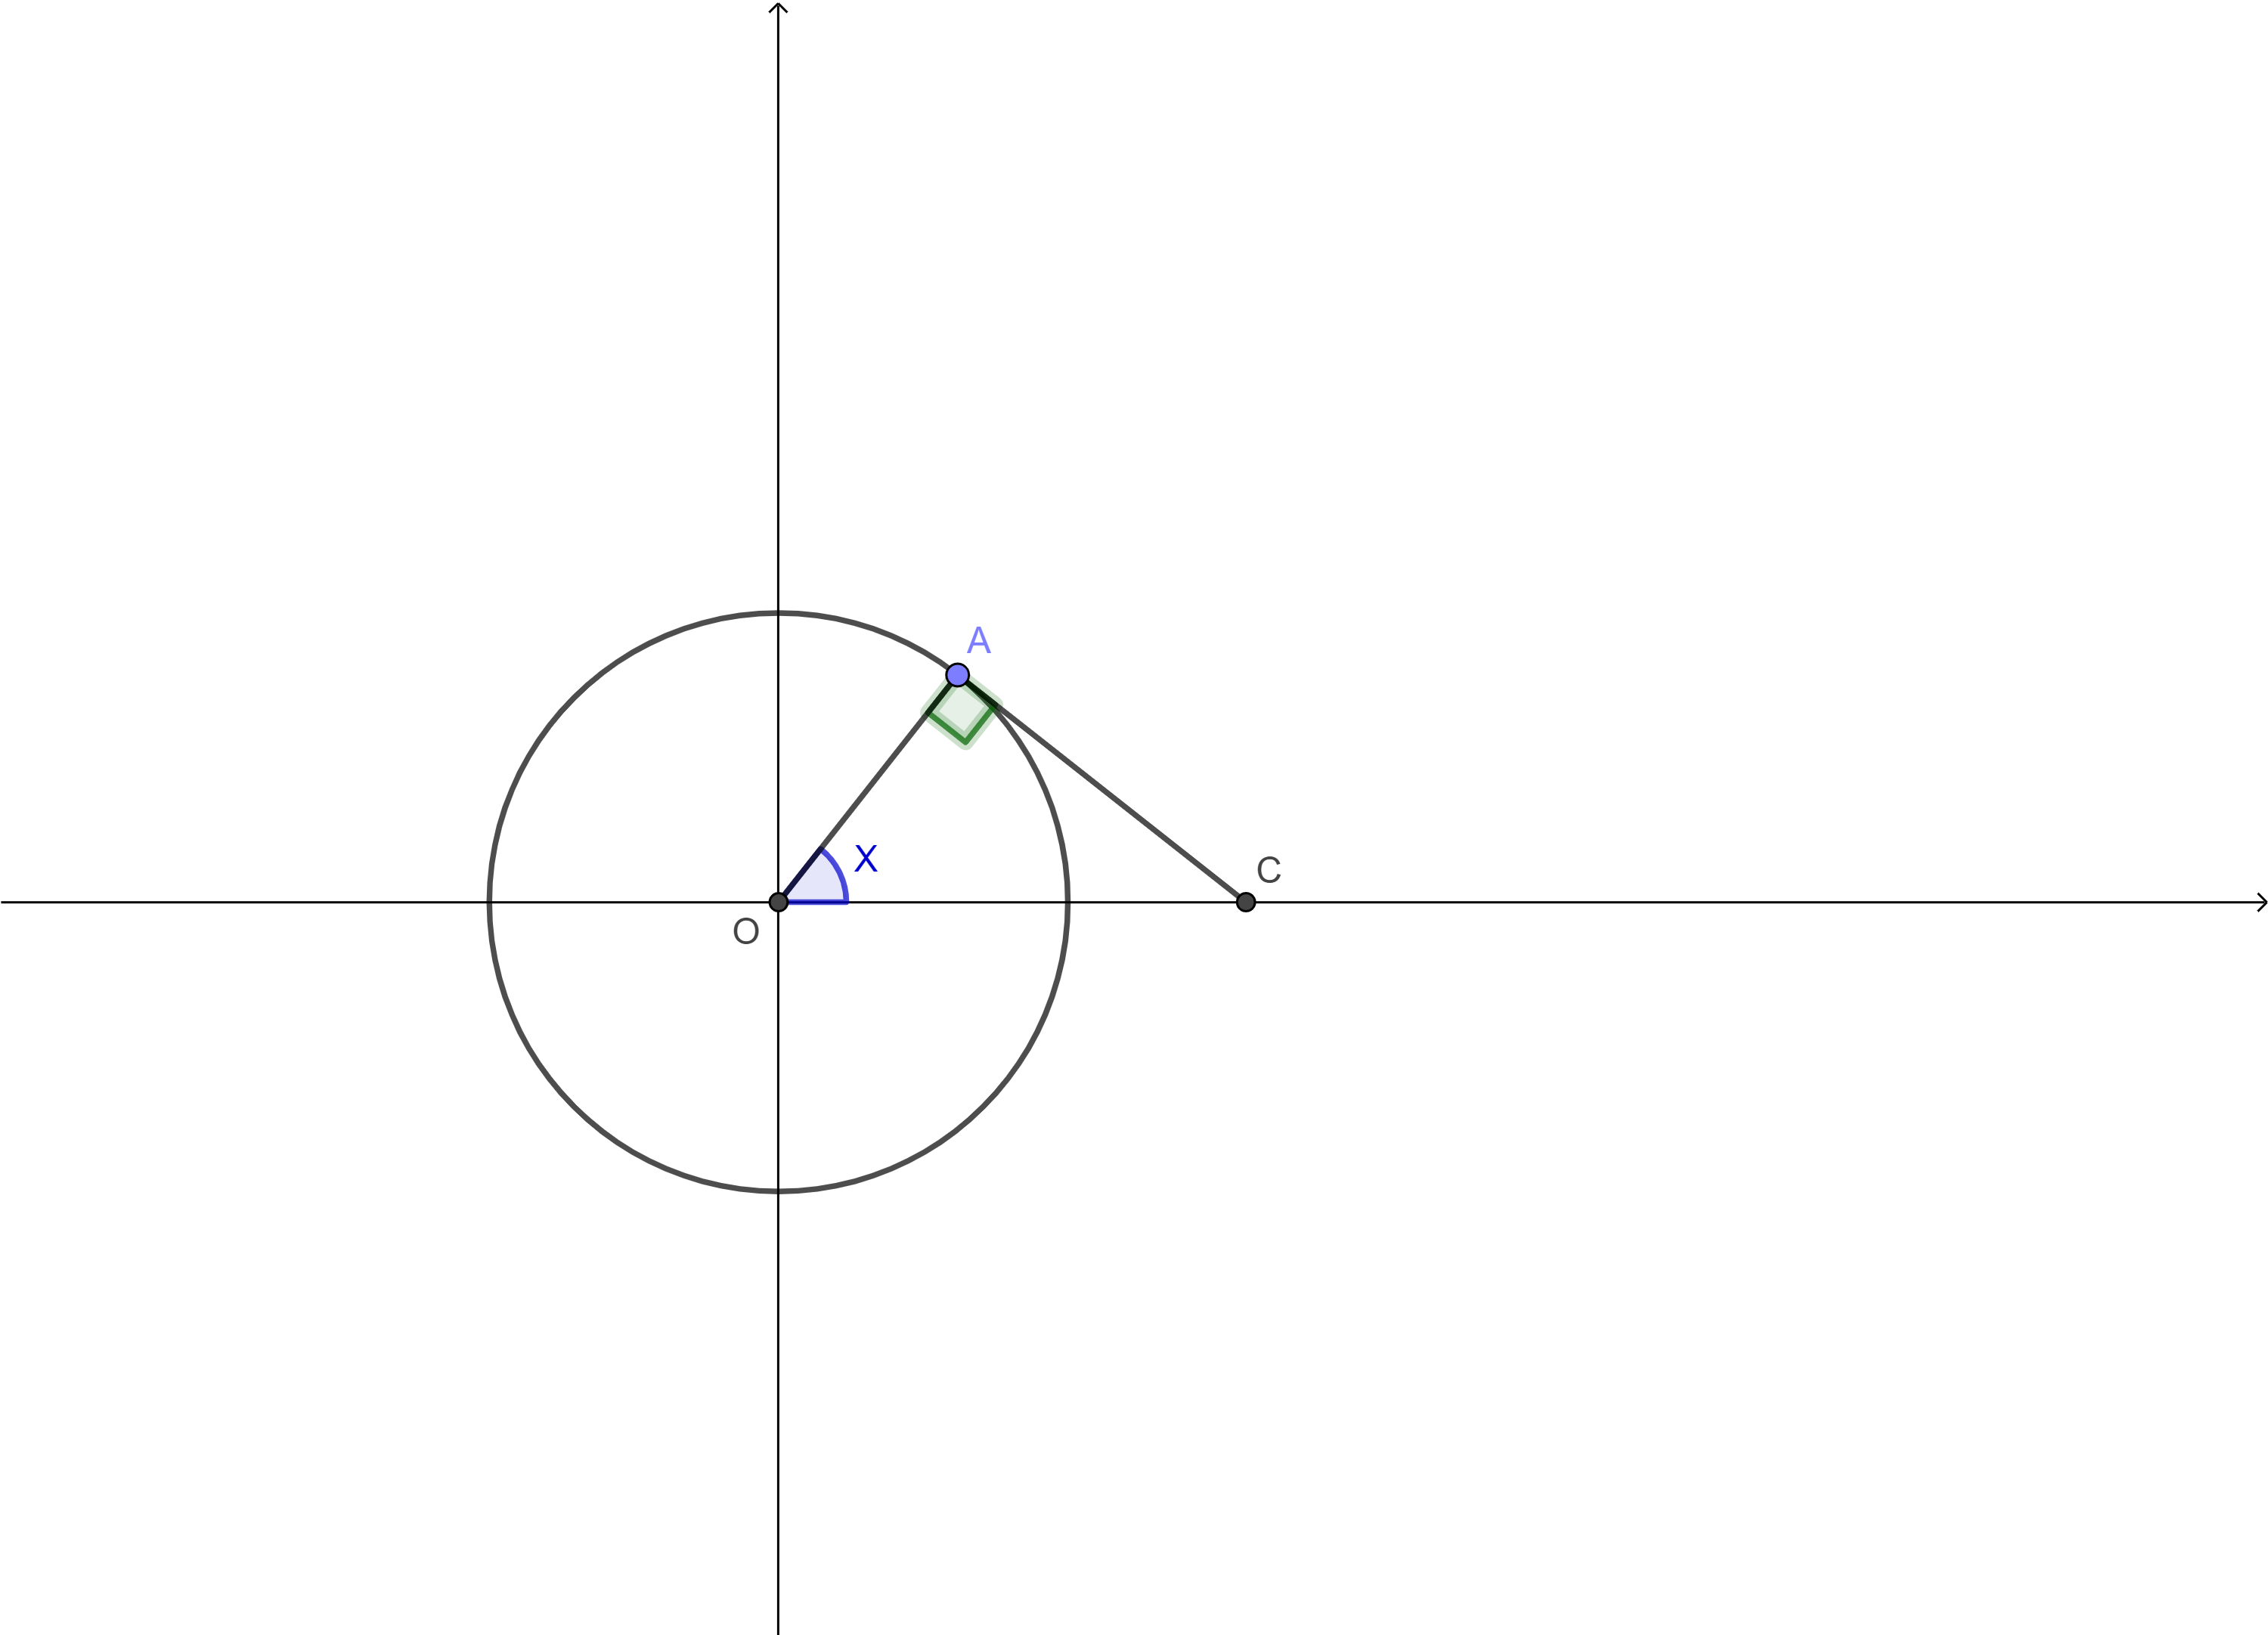
\includegraphics{exercise4-8.png}
	\centering
	\end{figure}

У нас есть $H=\tg X$, $x \in [0, \pi/2]$. Следовательно, $X$ имеет равномерное на $[0, \pi/2]$ распределения с функцией плотности вероятности $f(x)=\frac{2}{\pi}$. Поэтому $x = \arctg h$, $h \geq 0$

Мы получим $g(h)=\frac{2}{\pi} \cdot \Big|(\arctg h)'\Big| = \frac{2}{\pi \sqrt{1+h^2}}$, $h > 0$

При $h \leq 0$, $$F(h) = \int_{-\infty}^{h}0\,dh = 0$$

При $h > 0$, $$F(h) = \int_{-\infty}^{h}g(h)\,dh = \int_{0}^{h}\frac{2}{\pi \sqrt{1+h^2}}\,dh = \frac{2}{\pi} \cdot \arctg h$$
\end{exercise}

\begin{exercise}[5]
	Случайная величина $X$ равномерно распределения на отрезке $[0, 1]$, поэтому функция плотности вероятности $f(x)=1$
	
	У нас есть $Y=\ln(1/X) \Rightarrow y=\varphi(x)=\ln(1/x) \Rightarrow e^y = 1/x \Rightarrow x = 1/e^y$, $y \geq 0$
	
	Функция плотности вероятности случайной величины $Y$: $$g(h) = 1 \cdot \Big|(1/e^y)'\Big| = 1/e^y$$
	
	Тогда функция распределения:
	
	При $y<0$, $F(y)=0$
	
	При $y \geq 0$, $F(y) = \int_{-\infty}^{y}\,dy = \int_{0}^{y}1/e^y\,dy = -e^{-y}\Big|^y_0=-e^{-y} + e^0 = 1 - e^{-y}$
\end{exercise}

\begin{exercise}[6]
	$Y=X^2-X+1$
	\begin{itemize}
		\item $X=1$, $Y=1^2-1+1=1$
		\item $X=2$, $Y=2^2-2+1=3$
		\item $X=4$, $Y=4^2-4+1=13$
	\end{itemize}
	\begin{center}
		\begin{tabular}{|c|c|c|c|}
			\hline
			$Y$ & 1 & 3 & 13 \\ \hline
			$P$ & 0,3 & 0,5 & 0,2 \\ \hline
		\end{tabular}
	\end{center}
	Математическое ожидание $M\xi = 1 \cdot 0,3 + 3 \cdot 0,5 + 13 \cdot 0,2 = 4,4$
\end{exercise}

\begin{exercise}[7]
	Так как $X$ - число выпавших гербов при трех подбрасываниях монеты, вероятность равна по формуле Бернулли с $n=3$, $p=1/2$
	\begin{itemize}
		\item $X=0$, $P_3(X=0) = C^0_3 (1/2)^0 \cdot (1/2)^3=1/8$ и $Y=X^2=0$
		\item $X=1$, $P_3(X=1) = C^1_3 (1/2)^1 \cdot (1/2)^2 = 3/8$ и $Y=X^2=1$
		\item $X=2$, $P_3(X=2) = C^2_3 (1/2)^2 \cdot (1/2)^1 = 3/8$ и $Y=X^2=4$
		\item $X=3$, $P_3(X=3) = C^1_3 (1/2)^3 \cdot (1/2)^0 = 1/8$ и $Y=X^2=9$
	\end{itemize}
	Математическое ожидание случайной величины $Y$
	$$M\xi = 0 \cdot (1/8) + 1 \cdot (3/8) + 4 \cdot (3/8) + 9 \cdot (1/8) = 3$$
\end{exercise}

\begin{exercise}[8]
	Случайная величина $X$ равномерно распределения на отрезке $[0, 1] \Rightarrow$ функция распределения $f(x)=1$
	
	Мы найдем область значений $y=\varphi(x)$
	
	$Y=\sin(\pi X) \Rightarrow y = \varphi(x) = \sin(\pi x) \Rightarrow y' = \pi\cos(\pi x)$
	
	Если $y'=0 \Leftrightarrow \pi\cos(\pi x)=0 \Leftrightarrow \pi x = \pi/2 \Leftrightarrow x = 1/2$
	
	\begin{tikzpicture}
		\tkzTabInit{$x$ /1, $\varphi'(x)$ /1, $\varphi(x)$ /1}{$0$, $\frac{1}{2}$, $1$}
		\tkzTabLine{,+,z,-,}
		\tkzTabVar{-/$0$,+/$1$,-/$0$}
	\end{tikzpicture}

	Поэтому $y \in [0,1]$ и 
	\[
	x = \begin{cases}
		\frac{\arcsin y}{\pi} & \text{, при } x \in [0,1/2] \\ \frac{\pi - \arcsin y}{\pi} & \text{, при } x \in [1/2, 1] 
	\end{cases}
	\]
	
	Функция плотности вероятности случайной величины $Y$:
	$$g(y) = 1 \cdot \Big|\Big(\frac{\arcsin y}{\pi}\Big)'\Big| + 1 \cdot \Big|\Big(\frac{\pi - \arcsin y}{\pi}\Big)'\Big| = \frac{2}{\pi \sqrt{1-y^2}}$$
	
	Математическое ожидание
	$$M\xi = \int_{0}^{1}y \cdot \frac{2}{\pi \sqrt{1-y^2}} \,dy = \int_{0}^{1} \frac{-1}{\pi \sqrt{1-y^2}}\,d(1-y^2) = \frac{-2\sqrt{1-y^2}}{\pi}\Big|^1_0 = \frac{2}{\pi}$$
\end{exercise}

\begin{exercise}[9]
	$f(x)=0,5\sin x$ при $x \in [0, \pi]$ и $f(x)=0$ при остальных $x$ \\ У нас есть $Y = 2X \Rightarrow y = \varphi(x) = 2x \Rightarrow x = y/2$ при $y \in [0, 2\pi]$ \\ Функция плотности вероятности равна
	
	$g(y) = 0,5\sin (y/2) \cdot \Big|(y/2)'\Big|=0,25 \sin(y/2)$ при $y \in [0, 2\pi]$ и $f(y)=0$ при остальных $y$ \\ Математическое ожидание 
	\begin{align*}
		M\xi & = \int_{-\infty}^{+\infty}y \cdot g(y)\,dy \\ & = \int_{0}^{2\pi} 0,25 y\sin(y/2)\,dy \\ & = 0,25\int_{0}^{2\pi}y (-2\cos(y/2))' \,dy \\ & = 0,25 \Big[-2y\cos(y/2)\Big|^{2\pi}_0 - \int_{0}^{2\pi}1 \cdot (-2\cos(y/2)\,dy)\Big] \\ & = 0,25\Big[4\pi + 4\sin(y/2)\Big|^{2\pi}_0\Big] \\ & = 0,25\Big[4\pi + 0\Big] = \pi
	\end{align*}
\end{exercise}

\begin{exercise}[10]
	$f(x)=\frac{1}{\sqrt{2\pi}} e^{-x^2/2}$, при $x \in \mathbb{R}$ \\ У нас есть $Y=\frac{1}{2} X^2 \Rightarrow |x|=\sqrt{2y}$ и $y \geq 0$
	\begin{itemize}
		\item При $x<0$, $x = x_1(y) = -\sqrt{2y}$
		\item при $x\geq 0$, $x = x_2(y) = \sqrt{2y}$
	\end{itemize}
	Функция плотности вероятности
	\begin{align*}
		g(y) & = f(x_1(y))\cdot \Big|(-\sqrt{2y})'\Big| + f(x_2(y)) \cdot \Big|(\sqrt{2y})'\Big| \\ & = \frac{1}{\sqrt{2\pi}}e^{-y} \cdot \Big|\frac{-1}{\sqrt{2y}}\Big| + \frac{1}{\sqrt{2\pi}}e^{-y} \cdot \Big|\frac{1}{\sqrt{2y}}\Big| \\ & = \frac{2}{\sqrt{2\pi} \cdot \sqrt{2y}} e^{-y} = \frac{1}{\sqrt{\pi y}} e^{-y}
	\end{align*}
\end{exercise}

\begin{exercise}[11]
	$f(x) = \lambda e^{-\lambda x}$, $\lambda > 0$, $x \geq 0$ \\ У нас есть \\ $Y=\varphi(x)$, где $\varphi (x)=0,5x$ при $x \in [0,4]$ и $\varphi \equiv 2$ при $x \in (4, +\infty)$
	
	\begin{itemize}
		\item При $x \in [0, 4]$, $x=x(y)=2y$, $y \in [0,2]$
		\item При $x \in (4, +\infty)$, $y \equiv 2$
	\end{itemize}
	Поэтому $y=0$ при $y \not\in [0, 2]$ и если $y=2 \Rightarrow x=4$ 
	$$\Rightarrow P(Y=2) = \int_{4}^{+\infty} \lambda e^{-\lambda x}\,dx = -e^{-\lambda x}\Big|^{+\infty}_4 = 0 + e^{-4\lambda}$$
	
	$g(y) = f(x(y)) \Big|(2y)'\Big| + P(Y=2) \cdot \delta(y-2) = 2 \lambda e^{-2\lambda y} + e^{-4\lambda}\delta(y-2)$
\end{exercise}

\begin{exercise}[12]
	$f(x)=\frac{1}{\sqrt{2\pi}}\exp\Big(-\frac{x^2}{2}\Big)$ \\ У нас есть $Y=\varphi(X)$, где $\varphi(x)=0$ при $x<0$ и $\varphi(x) = 2x$ при $x \geq 0$
	
	$P(Y=0) = P(-\infty < X < 0) = \frac{1}{2}$ (свойства стандартного нормального распределения)
	
	У нас также есть: при $x \geq 0$, $x = \frac{y}{2}$
	
	Поэтому
	\begin{align*}
		g(y) & = \frac{1}{\sqrt{2\pi}}\exp\Big(-\frac{y^2}{4 \cdot 2}\Big) \cdot \Big|\Big(\frac{y}{2}\Big)'\Big| + P(Y=0) \cdot \delta(y-0) \\ & = \frac{1}{2\sqrt{2\pi}} \exp\Big(-\frac{y^2}{8}\Big) + \frac{1}{2} \delta(y)
	\end{align*}
\end{exercise}
	\newpage
	\section*{Занятие 9}
\begin{exercise}[1]
	\begin{table}[h]
		\centering
		\begin{tabular}{|c|c|c|c|}
			\hline
			$X$ & $Y$ & $Z$ & $P$ \\ \hline
			$2$ & $4$ & $6$ & $0,3 \cdot 0,4 = 0,12$ \\ \hline
			2 & 5 & 7 & \multirow{2}{*}{$0,3 \cdot 0,4 + 0,7 \cdot 0,4 = 0,46$} \\ \cline{1-3}
			3 & 4 & 7 & \\ \hline
			3 & 5 & 8 & $0,7 \cdot 0,6 = 0,42$ \\ \hline 
		\end{tabular}
		\begin{tabular}{|c|ccc|}
			\hline
			$Z$ & 6 & 7 & 8 \\ \hline
			$P$ & 0,12 & 0,46 & 0,42 \\ \hline
		\end{tabular}
	\caption{Занятие 9 - упражение 1}
	\end{table}
	$\Rightarrow M(Z) = 6 \cdot 0,12 + 7 \cdot 0,46 + 8 \cdot 0,42 = 7,3$
\end{exercise}

\begin{exercise}[2]
	$f(x) = \begin{cases}
		\lambda e^{-\lambda x} \text{ при } x \geq 0 \\
		0 \text{ при } x < 0
	\end{cases}$ \\
	$Z = X+Y \Rightarrow f(z) = \int_{-\infty}^{+\infty}f_1(x) f_2(z-x)\,dx$ \\
	При $z \geq 0 \Rightarrow f(z) = \int_{0}^{z}\lambda e^{-\lambda x} \cdot \lambda e^{-\lambda (z-x)}\,dx = \int_{0}^{z}\lambda^2 e^{-\lambda z}\,dx = \lambda^2 e^{-\lambda z}$ \\
	При $z < 0$, $f(z)=0$
\end{exercise}

\begin{exercise}[3]
	$Z=2X-Y+5$, $M(X)=3$, $M(Y)=5$, $D(X)=2$, $D(Y)=1$ \\
	$M(Z)=2M(X)-M(Y)+5=6$ \\
	$D(Z)=D(2X)+D(Y)=4D(X)+D(Y)=9=\sigma^2 \Rightarrow \sigma=3$
\end{exercise}

\begin{exercise}[4]
	$X$ и $Y$ независимы. $f_1(x) = f_2(y) = \frac{1}{2}$. $X, Y ~ U(0, 2)$. $Z=X+Y$ \\
	При $0 \leq z < 2$, $f(z) = \int_{0}^{z}\frac{1}{2} \cdot \frac{1}{2}\,dx = \frac{z}{4}$ \\
	При $2 \leq z < 4$, $f(z) = \int_{z-2}^{2}\frac{1}{2} \cdot \frac{1}{2}\,dx = \frac{1}{4}(2-z+2) = 1-0,25z$ \\
	При остальных $z$, $f(z)=0$
\end{exercise}

\begin{exercise}[6]
	Св $X$ и $Y$ независимы, равномерно на $(0, 1)$. $Z=Y/X^2$
	
	 У нас есть $F(z) = P(Z \leq z) = P(Y/X^2 \leq z)$, $y/x^2\leq z \Leftrightarrow y \leq zx^2$
	 \begin{itemize}
	 	\item При $z \leq 0$, $f(z)=0$
	 	\item При $0 < z \leq 1$, $F(z) = \int_{0}^{1}\,dx\int_{0}^{zx^2}\,dy = \int_{0}^{1}zx^2\,dx = \frac{z}{3}$ \\ $\Rightarrow f(z) = \frac{1}{3}$
	 	\item При $z > 1$, $y \leq zx^2 \Rightarrow x \geq \sqrt{\frac{y}{z}}$ \\ $\Rightarrow F(z) = \int_{0}^{1}\,dy \int_{\sqrt{y/z}}^{1}\,dx = \int_{0}^{1}(1 - \sqrt{\frac{y}{z}})\,dy=1-\frac{2}{3\sqrt{z}}$ \\ $\Rightarrow f(z) = 1/(3z^{1,5})$
	 \end{itemize}
\end{exercise}

\begin{exercise}[7]
	\textbf{$U=min(X, Y)$}
	\begin{itemize}
		\item При $u < 0$, $F(u)=0$
		\item При $0 \leq u < 1$, $F(u) = P(min(X, Y) \leq u) = 1 - P(min(X, Y) > u) = 1 - \int_{u}^{1}\int_{u}^{1}\,dx\,dy = 2u-u^2$
		\item При $u>1$, $F(u)=1$
	\end{itemize}
	$\Rightarrow M(U) = \int_{0}^{1}u(2-2u)\,du=1/3$ \\
	$\Rightarrow D(U) = \int_{0}^{1}(u-\frac{1}{3})^2(2-2u)\,du = 1/18$
	
	\textbf{$V=max(X, Y)$}
	\begin{itemize}
		\item При $v < 0$, $F(v) = 0$
		\item При $0 \leq v < 1$, $F(v) = P(max(X, Y) \leq v) = \int_{0}^{v}\int_{0}^{v}\,dx\,dy = v^2 \Rightarrow f(v) = 2v$
		\item При $v > 1$, $F(v)=1$
	\end{itemize}
	$\Rightarrow M(v) = \int_{0}^{1}v\cdot 2v\,dv = 2/3$ \\
	$\Rightarrow D(v) = \int_{0}^{1}(v-\frac{2}{3})^2\cdot 2v\,dv = 1/18$
\end{exercise}

\begin{exercise}[9]
	Площадь треугольника $ABC$ равна 1 $\Rightarrow f(x, y) = 1$ \\ $y \leq \frac{x}{2} \Rightarrow \begin{cases}
		0 \leq y \leq \frac{x}{2} \\ 2y \leq x \leq 2
	\end{cases}$ \\ $f_1(x) = \int_{0}^{x/2}1\,dy = \frac{2}{x}$ \\ $f_2(y) = \int_{2y}^{2}1\,dx = 2-2y$ \\ $M(X) = \int_{0}^{2}x \cdot \frac{x}{2}\,dx = \frac{4}{3}$, $M(X^2) = \int_{0}^{2}x^2 \cdot \frac{x}{2}\,dx = 2$ \\ $M(Y) = \int_{0}^{1}y(2-2y)\,dy = \frac{1}{3}$,  $M(Y^2) = \int_{0}^{1}y^2(2-2y)\,dy=\frac{1}{6}$ \\ $M(\overset{\circ}{X}\cdot \overset{\circ}{Y}) = \int_{0}^{2}\,dx\int_{0}^{x/2}(x-\frac{4}{3})(y-\frac{1}{3})\,dy = \cdots = \frac{1}{18}$ \\ $\sigma_x^2 = M(X^2)-M(X)^2=2-\frac{16}{9}=\frac{2}{9}$ \\ $\sigma_y^2 = M(Y^2)-M(Y)^2=\frac{1}{6} - \frac{1}{9} = \frac{1}{18}$ \\ $\Rightarrow r_{xy} = \frac{1}{2}$

	Линия регрессии: $\frac{y-1/3}{\sigma_y} = r_{xy}\frac{x-4/3}{\sigma_x} \Rightarrow y = \frac{x}{4}$
\end{exercise}

\begin{exercise}[11]
	$f(x) \rightarrow g(y)$, $Y = min(X, X^2)$. У нас есть
	\begin{itemize}
		\item При $x<0$ или $x \geq 1$, $min(X, X^2)=X$
		\item При $0 \leq x < 1$, $min(X, X^2)=X^2$
	\end{itemize}
	$G(y) = P(Y \leq y) = P(min(X, X^2) \leq y)$
	\begin{itemize}
		\item При $y < 0$, $G(y) = P(X \leq y) = \int_{-\infty}^{y}f(x)\,dx = F(y) \Rightarrow g(y)=f(y)$
		\item При $0 \leq y < 1$, $G(y) = P(X^2 \leq y) = P(X \leq \sqrt{Y}) = \int_{0}^{\sqrt{y}}f(x)\,dx = F(\sqrt{y}) \Rightarrow g(y) = f(\sqrt{y})(\sqrt{y})'=\frac{f(\sqrt{y})}{2\sqrt{y}}$
		\item При $y \geq 1$, $G(y) = P(X \leq y) = \int_{1}^{y}f(x)\,dx = F(y) \Rightarrow g(y)=f(y)$
	\end{itemize}
\end{exercise}

\begin{exercise}[12]
	$X_1, X_2 \rightarrow f(x_1, x_2) = \frac{2}{\pi^2(x_1^2+1)(x_2^2+4)}$, $g(y_1, y_2) \rightarrow Y_1, Y_2$, $X_1 = \tg(Y_1)$, $X_2 = 2\tg(Y_2)$, $|Y_1|<\pi/2$, $|Y_2|<\pi/2$
	
	При $|y_1| < \pi/2$, $|y_2| < \pi/2$
	\begin{align*}
		G(y_1, y_2) & = P(Y_1 \leq y_1, Y_2 \leq y_2) \\
		& P(\arctg(X_1) \leq y_1, \arctg(\frac{X_2}{2}) \leq y_2) \\ & P(X_1 \leq \tg(y_1), X_2 \leq 2\tg(y_2)) \\ & \int_{-\infty}^{\tg y_1}\int_{-\infty}^{2\tg y_2}\frac{2\,dx_1\,dx_2}{\pi^2(x_1^2+1)(x_2^2+4)} \\ & \int_{-\infty}^{\tg y_1}\,dx_1\cdot \frac{2}{\pi^2(x_1^2+1)} \cdot \frac{1}{2} \arctg(\frac{x_2}{2})\Big|^{2\tg y_2}_{-\infty} \\ & \int_{-\infty}^{\tg y_1}(y_2 + \frac{\pi}{2})\frac{\,dx_1}{\pi^2(x_1^2+1)} \\ & \frac{1}{\pi^2}(y_1+\frac{\pi}{2})(y_2 + \frac{\pi}{2})
	\end{align*}
	$\Rightarrow g(y_1, y_2) = \frac{\partial^2G(y_1, y_2)}{\partial y_1 \partial y_2} = \frac{1}{\pi^2}$
	
	При остальных $y_1$, $y_2$, $g(y_1, y_2) = 0$
\end{exercise}
	\newpage
	\textbf{Ещё не решил}:
	\begin{itemize}
		\item Занятие 3: 7б, 10
		\item Занятие 5: 2, 8
		\item Занятие 8: 13
		\item Занятие 9: 5
	\end{itemize}
	\newpage
	\section*{КМ 2 - 07/04/2021}
\subsection*{Вариант 1}
\begin{exercise}[1] Вероятность того, что радиоприемник проработает гарантийный срок без отказов равна 0,9. Какова вероятность того, что из данных пяти радиоприемников три проработают гарантийный срок без отказов?
	$n=5$, $p=0,9 \Rightarrow q = 1-p=0,1$ \\ Мы получим $P_5(3) = C^3_5 p^3 q^2 = C^3_5 \cdot (0,9)^3 \cdot (0,1)^2 = 0,0729$
\end{exercise}
\begin{exercise}[2] Студент знает 20 из 25 вопросов программы. Студенту предлагается три вопроса. Какова вероятность того, что студент знает только один из предложенных ему вопросов? Какова вероятность того, что студент знает ответы на все три предложенных ему вопроса?
	
	$| \Omega | = C^3_{25}$ \\ Пусть $A$ = \{студент знает только один из предложенных\} \\ Выбрать 1 вопрос, который студент знает $\Rightarrow C^1_{20}$ вариантов \\ Выбрать 2 вопрос, которые студент не знает $\Rightarrow C^2_5$ вариантов \\ $\Rightarrow P(A) = \frac{C^1_{20} C^2_5}{C^3_{25}} = \frac{2}{23}$ \\ $B$ = \{студент знает все 3 вопроса\} \\ $P(B) = \frac{C^3_{20}}{C^3_{25}} = \frac{57}{115}$
\end{exercise}

\begin{exercise}[3] В двух урнах находятся шары отличающиеся только цветом причем в первой урне 5 белых, 11 черных и 6 красных шаров, а во второй соответственно 10, 8, 6. Из каждой урны извлекли по одному шару. Какова вероятность того, что оба шара одного цвета?
	
	$|\Omega| = C^1_{5+11+6} C^1_{10 + 8 + 6} = C^1_{22} C^1_{24}$ \\ Пусть $A$ = \{оба шара одного цвета\}. У нас есть 3 случая
	\begin{itemize}
		\item белый: $C^1_5 C^1_{10}$ вариантов
		\item черный: $C^1_{11} C^1_8$ вариантов
		\item красный: $C^1_6 C^1_6$ вариантов
	\end{itemize}
	Ответ $P(A) = \frac{C^1_5 C^1_{10} + C^1_{11} C^1_8 + C^1_6 C^1_6}{C^1_{22} C^1_{24}} = \frac{29}{88}$
\end{exercise}

\begin{exercise}[4] В одном из двух ящиков лежит  3  белых и  7  черных шаров, а в другом лежит 5  белых  и   4   черных шара. Наугад выбирается один из ящиков и вынимается из него шар, который оказался белым. Найти вероятность того, что следующий извлеченный из этого же ящика шар тоже белый.

Пусть $A_1$ = \{первый ящик выбирается\} \\ $A_2$ = \{второй ящик выбирается\} \\ $A$ = \{первый шар - белый\} \\ $\Rightarrow P(A) = P(A_1) P(A | A_1) + P(A_2) P(A | A_2) = \frac{1}{2} \cdot \frac{3}{10} + \frac{1}{2} \cdot \frac{5}{9} = \frac{77}{180}$ \\ Отсюда, если пусть $B_1$ = \{первый белый шар из первого ящика\} \\ $B_2$ = \{первый белый шар из второго ящика\} \\ $B$ = \{второй шар - белый\} \\ мы получим
\begin{align*}
	P(B_1) & = P(A_1 | A) = \frac{1/2 \cdot 3/10}{77/180} = \frac{27}{77} \\ P(B_2) & = P(A_2 | A) = \frac{1/2 \cdot 5/9}{77/180} = \frac{50}{77}
\end{align*}
Если первый ящик выбирается, после мы взяли один белый шар, еще 8 белых, тогда $P(B | B_1) = \frac{2}{9}$. Аналогично, $P(B | B_2) = \frac{4}{8}$ \\ $\Rightarrow P(B) = P(B_1) P(B | B_1) + P(B_2) P(B | B_2) = \frac{27}{77} \cdot \frac{2}{9} + \frac{50}{77} \cdot \frac{4}{8} = \frac{31}{77}$
\end{exercise}

\begin{exercise}[5] Имеется  5 ящиков, в каждом из которых   10  белых  и  30  черных шаров. Из первого ящика во второй перекладывается один шар, затем из второго в третий перекладывается один шар  и т.д. После чего из последнего ящика извлекается один шар. Найти вероятность того, что он белый.

Пусть $A_1$ = \{белый шар из 1-ого ящика\} $\Rightarrow \overline{A_1}$ = \{черный шар из 1-ого ящика\} \\ $A_2$ = \{белый шар из 2-ого ящика\} $\Rightarrow \overline{A_2}$ = \{черный шар из 2-ого ящика\} \\ $A_3$ = \{белый шар из 3-ого ящика\} $\Rightarrow \overline{A_3}$ = \{черный шар из 3-ого ящика\} \\ $A_4$ = \{белый шар из 4-ого ящика\} $\Rightarrow \overline{A_4}$ = \{черный шар из 4-ого ящика\} \\ $A_5$ = \{белый шар из 5-ого ящика\} $\Rightarrow \overline{A_5}$ = \{черный шар из 5-ого ящика\}

Если мы выбираем белый шар из $i$-ого ящика, тогда в $i+1$-ом ящике есть 8+1=9 белых ящиков. Значит $P(A_{i+1} | A_i) = \frac{11}{41}$. Аналогично, если мы выбираем черный шар из $i$-ого ящика, $P(A_{i+1} | \overline{A_i}) = \frac{10}{41}$ и $$P(A_{i+1}) = P(A_i) P(A_{i+1} | A_i) + P(\overline{A_i}) P(A_{i+1} | \overline{A_i})$$ 

$P(A_1) = \frac{10}{40} = \frac{1}{4}$, $P(\overline{A_1}) = \frac{30}{40} = \frac{3}{4}$ \\ $\Rightarrow P(A_2) = P(A_1) P(A_2 | A_1) + P(\overline{A_1}) P(A_2 | \overline{A_1}) = \frac{1}{4} \cdot \frac{11}{41} + \frac{3}{4} \cdot \frac{10}{41} = \frac{1}{4}$ \\ $\Rightarrow P(\overline{A_2}) = 1-1/4=3/4$ \\ Аналогично, $P(A_2) = P(A_3) = P(A_4) = P(A_5) = \frac{1}{4}$ \\ Ответ $\frac{1}{4}$
\end{exercise}

\subsection*{Вариант 22}
\begin{exercise}[1] Из колоды карт (36 штук) выбирают наугад две карты. Какова вероятность того, что обе они окажутся пиковой масти?
	
	У нас есть 36 карт и выбирать 2 карты $\Rightarrow | \Omega | = C^2_{36}$ \\ Пусть $A$ = \{обе они окажутся пиковой масти\} \\ В колоде карт есть 9 пиковых мастей $\Rightarrow | \Omega_A | = C^2_9$ \\ $\Rightarrow P(A) = \frac{C^2_9}{C^2_{36}} = \frac{2}{35}$
\end{exercise}

\begin{exercise}[2] Из урны, содержащей пять белых и четыре черных шара, извлекают шары по одному без возвращения, пока не будет извлечен белый шар. Какова вероятность того, что придется извлечь четыре шара?
	
	Пусть $A_i$ = \{выбрать $i$ черных шаров, пока не будет извлечен белый шар\} $\Rightarrow i \in \{0, 1, 2, 3, 4\}$ \\ $B$ = \{выбрать белый шар в последний раз\} \\ У нас есть $P(B|A_0) = P(B|A_1) = \cdots = P(B|A_4) = \frac{1}{5}$
	\begin{align*}
		P(A_0) & = \frac{A^0_4}{A^0_9} = 1 \\ P(A_1) & = \frac{A^1_4}{A^1_9} = \frac{4}{9} \\ P(A_2) & = \frac{A^2_4}{A^2_9} = \frac{1}{6} \\ P(A_3) & = \frac{A^3_4}{A^3_9} = \frac{1}{21} \\ P(A_4) & = \frac{A^4_4}{A^4_9} = \frac{1}{126}
	\end{align*}
	\begin{align*}
		\Rightarrow P(A_3 | B) & = \frac{P(B|A_3)P(A_3)}{\sum_{i=0}^{4}P(B|A_i) P(A_i)} \\ & = \frac{1/5 \cdot 1/21}{1/5 \cdot (1 + 4/9 + 1/6 + 1/21 + 1/126)} = \frac{1}{35}
	\end{align*}
\end{exercise}

\begin{exercise}[3] Для каждого из чисел $X$ и $Y$ равновозможно любое значение из отрезка [0;2]. Какова вероятность того, что разность $X - Y$ превосходит единицу?
	
	У нас есть $X-Y \geq 1$ и $X, Y \in [0,2]$. Значит
	$\begin{cases}
		X - Y \geq 1 \\ 0 \leq X, Y \leq 2
	\end{cases}$
	Отсюда мы получим вероятность равно $P = \frac{S_{\triangle AB}}{S_{OBMN}} = \frac{1/2}{4} = \frac{1}{8}$
\end{exercise}

\begin{exercise}[4] В одном из двух ящиков лежит 9 белых и 3 черных шара, а в другом лежит 6 белых и 3 черных шара. Наугад выбирается один из ящиков и вынимается из него шар, который оказался белым. Найти вероятность того, что следующий извлеченный из этого же ящика шар тоже белый.
	
	Пусть $A_1$ = \{первый ящик выбирается\} \\ $A_2$ = \{второй ящик выбирается\} \\ $A$ = \{первый шар - белый\} \\ $\Rightarrow P(A) = P(A_1) P(A | A_1) + P(A_2) P(A | A_2) = \frac{1}{2} \cdot \frac{9}{12} + \frac{1}{2} \cdot \frac{6}{9} = \frac{17}{24}$ \\ Отсюда, если пусть $B_1$ = \{первый белый шар из первого ящика\} \\ $B_2$ = \{первый белый шар из второго ящика\} \\ $B$ = \{второй шар - белый\} \\ мы получим
	\begin{align*}
		P(B_1) & = P(A_1 | A) = \frac{1/2 \cdot 9/12}{17/24} = \frac{9}{17} \\ P(B_2) & = P(A_2 | A) = \frac{1/2 \cdot 6/9}{17/24} = \frac{8}{17}
	\end{align*}
	Если первый ящик выбирается, после мы взяли один белый шар, еще 8 белых, тогда $P(B | B_1) = \frac{8}{11}$. Аналогично, $P(B | B_2) = \frac{5}{8}$ \\ $\Rightarrow P(B) = P(B_1) P(B | B_1) + P(B_2) P(B | B_2) = \frac{9}{17} \cdot \frac{8}{11} + \frac{8}{17} \cdot \frac{5}{8} = \frac{127}{187}$
\end{exercise}

\begin{exercise}[5] Имеется  5 ящиков, в каждом из которых   8  белых  и  16  черных шаров. Из первого ящика во второй перекладывается один шар, затем из второго в третий перекладывается один шар  и т.д. После чего из последнего ящика извлекается один шар. Найти вероятность того, что он белый.
	Пусть $A_1$ = \{белый шар из 1-ого ящика\} $\Rightarrow \overline{A_1}$ = \{черный шар из 1-ого ящика\} \\ $A_2$ = \{белый шар из 2-ого ящика\} $\Rightarrow \overline{A_2}$ = \{черный шар из 2-ого ящика\} \\ $A_3$ = \{белый шар из 3-ого ящика\} $\Rightarrow \overline{A_3}$ = \{черный шар из 3-ого ящика\} \\ $A_4$ = \{белый шар из 4-ого ящика\} $\Rightarrow \overline{A_4}$ = \{черный шар из 4-ого ящика\} \\ $A_5$ = \{белый шар из 5-ого ящика\} $\Rightarrow \overline{A_5}$ = \{черный шар из 5-ого ящика\}
	
	Если мы выбираем белый шар из $i$-ого ящика, тогда в $i+1$-ом ящике есть 8+1=9 белых ящиков. Значит $P(A_{i+1} | A_i) = \frac{9}{25}$. Аналогично, если мы выбираем черный шар из $i$-ого ящика, $P(A_{i+1} | \overline{A_i}) = \frac{8}{25}$ и $$P(A_{i+1}) = P(A_i) P(A_{i+1} | A_i) + P(\overline{A_i}) P(A_{i+1} | \overline{A_i})$$ 
	
	$P(A_1) = \frac{8}{24} = \frac{1}{3}$, $P(\overline{A_1}) = \frac{16}{24} = \frac{2}{3}$ \\ $\Rightarrow P(A_2) = P(A_1) P(A_2 | A_1) + P(\overline{A_1}) P(A_2 | \overline{A_1}) = \frac{1}{3} \cdot \frac{9}{25} + \frac{2}{3} \cdot \cdot \frac{8}{25} = \frac{1}{3}$ \\ $\Rightarrow P(\overline{A_2}) = 1-1/3=2/3$ \\ Аналогично, $P(A_2) = P(A_3) = P(A_4) = P(A_5) = \frac{1}{3}$ \\ Ответ $\frac{1}{3}$
\end{exercise}
\end{document}